%%%%%%%%%%%%%%%%%%%%%%%%%%%%%%%%%%%%%%%%%
% Masters/Doctoral Thesis 
% LaTeX Template
% Version 2.5 (27/8/17)
%
% This template was downloaded from:
% http://www.LaTeXTemplates.com
%
% Version 2.x major modifications by:
% Vel (vel@latextemplates.com)
%
% This template is based on a template by:
% Steve Gunn (http://users.ecs.soton.ac.uk/srg/softwaretools/document/templates/)
% Sunil Patel (http://www.sunilpatel.co.uk/thesis-template/)
%
% Template license:
% CC BY-NC-SA 3.0 (http://creativecommons.org/licenses/by-nc-sa/3.0/)
%
%%%%%%%%%%%%%%%%%%%%%%%%%%%%%%%%%%%%%%%%%

%----------------------------------------------------------------------------------------
%	PACKAGES AND OTHER DOCUMENT CONFIGURATIONS
%----------------------------------------------------------------------------------------

\documentclass[
11pt, % The default document font size, options: 10pt, 11pt, 12pt
%oneside, % Two side (alternating margins) for binding by default, uncomment to switch to one side
english, % ngerman for German
singlespacing, % Single line spacing, alternatives: onehalfspacing or doublespacing
%draft, % Uncomment to enable draft mode (no pictures, no links, overfull hboxes indicated)
%nolistspacing, % If the document is onehalfspacing or doublespacing, uncomment this to set spacing in lists to single
%liststotoc, % Uncomment to add the list of figures/tables/etc to the table of contents
%toctotoc, % Uncomment to add the main table of contents to the table of contents
parskip, % Uncomment to add space between paragraphs
%nohyperref, % Uncomment to not load the hyperref package
headsepline, % Uncomment to get a line under the header
%chapterinoneline, % Uncomment to place the chapter title next to the number on one line
%consistentlayout, % Uncomment to change the layout of the declaration, abstract and acknowledgements pages to match the default layout
]{master-thesis} % The class file specifying the document structure
\restoreparindent
\usepackage[utf8]{inputenc} % Required for inputting international characters
\usepackage[T1]{fontenc} % Output font encoding for international characters
\usepackage{amsmath}
\usepackage{hyperref}
%\usepackage{mathpazo} % Use the Palatino font by default
%\usepackage{xfrac,unicode-math}
\usepackage[eng,exjobb]{KTHEEtitlepage}
\usepackage{amssymb}
\usepackage{bm}
\usepackage{cancel}
\usepackage{booktabs, lscape}

\usepackage[backend=bibtex,style=authoryear,natbib=true]{biblatex} % Use the bibtex backend with the authoryear citation style (which resembles APA)
%\setlength{\intextsep}{10pt plus 1.0pt minus 2.0pt}
\addbibresource{biblio.bib} % The filename of the bibliography
\usepackage{float}
\usepackage[autostyle=true]{csquotes} % Required to generate language-dependent quotes in the bibliography
\usepackage{subcaption}
\newcommand{\overbar}[1]{\mkern 1.5mu\overline{\mkern-1.5mu#1\mkern-1.5mu}\mkern 1.5mu}
%\setmathfont{Latin Modern Math}[version=lm]
\newcommand{\ra}[1]{\renewcommand{\arraystretch}{#1}}

%----------------------------------------------------------------------------------------
%	MARGIN SETTINGS
%----------------------------------------------------------------------------------------

\geometry{
	paper=a4paper, % Change to letterpaper for US letter
	inner=2.5cm, % Inner margin
	outer=3.5cm, % Outer margin
	bindingoffset=.5cm, % Binding offset
	top=1.5cm, % Top margin
	bottom=1.5cm, % Bottom margin
	%showframe, % Uncomment to show how the type block is set on the page
}

%----------------------------------------------------------------------------------------
%	THESIS INFORMATION
%----------------------------------------------------------------------------------------

\thesistitle{Energy-based Multi-Modal Attention} % Your thesis title, this is used in the title and abstract, print it elsewhere with \ttitle
\supervisor{Dr. Raphaël \textsc{Marée}} % Your supervisor's name, this is used in the title page, print it elsewhere with \supname
\examiner{} % Your examiner's name, this is not currently used anywhere in the template, print it elsewhere with \examname
\degree{Master of Computer Science and Engineering} % Your degree name, this is used in the title page and abstract, print it elsewhere with \degreename
\author{Aurélien \textsc{Werenne}} % Your name, this is used in the title page and abstract, print it elsewhere with \authorname
\addresses{} % Your address, this is not currently used anywhere in the template, print it elsewhere with \addressname

\subject{Artificial Intelligence} % Your subject area, this is not currently used anywhere in the template, print it elsewhere with \subjectname
\keywords{Multimodal, Deep Learning, Attention, Robustness} % Keywords for your thesis, this is not currently used anywhere in the template, print it elsewhere with \keywordnames
\university{University of Liège} % Your university's name and URL, this is used in the title page and abstract, print it elsewhere with \univname
\faculty{Faculty of Applied Sciences} % Your faculty's name and URL, this is used in the title page and abstract, print it elsewhere with \facname
\department{Montefiore Institute} % Your department's name and URL, this is used in the title page and abstract, print it elsewhere with \deptname
\group{\href{http://www.montefiore.ulg.ac.be/systmod/}{Systems and Modelling}} % Your research group's name and URL, this is used in the title page, print it elsewhere with \groupname

\AtBeginDocument{
\hypersetup{pdftitle=\ttitle} % Set the PDF's title to your title
\hypersetup{pdfauthor=\authorname} % Set the PDF's author to your name
\hypersetup{pdfkeywords=\keywordnames} % Set the PDF's keywords to your keywords
}

\begin{document}

\frontmatter % Use roman page numbering style (i, ii, iii, iv...) for the pre-content pages

\pagestyle{plain} % Default to the plain heading style until the thesis style is called for the body content

%----------------------------------------------------------------------------------------
%	TITLE PAGE
%----------------------------------------------------------------------------------------
\ititle{Energy-based Multi-Modal Attention}
\idate{August 2019}
\color{white}\iauthor{Aurelien Werenne}
\makeititle
\color{black}
\begin{titlepage}
\begin{center}

%\vspace*{.06\textheight}
%{\scshape\LARGE \univname\par}\vspace{1.5cm} % University name
%\textsc{\Large Master Thesis}\\[0.5cm] % Thesis type

\vspace*{.06\textheight}
\begin{center}

\includegraphics[scale=0.6]{figures/logo-uliege}\\[1.6cm] 
\end{center}

\HRule \\[0.4cm] % Horizontal line
{\huge \bfseries \ttitle\par}\vspace{0.4cm} % Thesis title
\HRule \\[1.5cm] % Horizontal line
 
\begin{minipage}[t]{0.4\textwidth}
\begin{flushleft} \large
\emph{Author:}\\
\authorname 
\end{flushleft}
\end{minipage}
\begin{minipage}[t]{0.4\textwidth}
\begin{flushright} \large
\emph{Supervisor:} \\
\supname
\end{flushright}
\end{minipage}\\[2.4cm]

\large \textit{A thesis submitted in partial fulfillment of the requirements\\ for the degree of \degreename}\\[1cm] % University requirement text
\deptname\\
\facname\\
\univname\\
Liège, Belgium\\[4cm] 
 

%\begin{center}
%
\includegraphics[scale=0.6]{figures/logo-uliege}\\[1.6cm] 
%\end{center}
{\large Academic Year 2018 - 2019}
 
\vfill
\end{center}
\end{titlepage}

%----------------------------------------------------------------------------------------
%	QUOTATION PAGE
%----------------------------------------------------------------------------------------

\vspace*{0.2\textheight}

\noindent\enquote{\itshape Sometimes it seems as though each new step towards Artificial Intelligence, rather than producing something which everyone agrees is real intelligence, merely reveals what real intelligence is not.}\bigbreak
\hfill Douglas Hofstadter
%\ldots

%----------------------------------------------------------------------------------------
%	ABSTRACT PAGE
%----------------------------------------------------------------------------------------

\begin{abstract}
\addchaptertocentry{\abstractname} % Add the abstract to the table of contents
A multi-modal neural network exploits information from different channels and in different terms (e.g., images, text, sounds, sensor measures) in the hope that the information carried by each mode is complementary, in order to improve the predictions of the neural network. Nevertheless, in realistic situations, varying levels of perturbations can occur on the data of the modes, which may decrease the quality of the inference process. An additional difficulty is that these perturbations vary between the modes and on a per-sample basis. This work presents a solution to this problem. The three main contributions are described below.

First, a novel attention module is designed, analysed and implemented. This attention module is constructed to help multi-modal networks handle modes with perturbations.

Secondly, two new regularizers are developed to generalize the robustness to more intensive failing modes (relative to the training set).

Lastly, a unified multi-modal attention module is presented, combining the main types of attention mechanisms in the deep learning literature with our module. We suggest that the unified module could be coupled with a prediction model to enable the latter face unexpected situations, and extract the most relevant information from the input data.

\end{abstract}

%----------------------------------------------------------------------------------------
%	ACKNOWLEDGEMENTS
%----------------------------------------------------------------------------------------

\begin{acknowledgements}
\addchaptertocentry{\acknowledgementname} % Add the acknowledgements to the table of contents
\vspace*{5mm}
I would like to thank everybody who kept me busy this year. In particular, my thesis advisor Dr. Raphaël Marée for always encouraging my research, and Romain Mormont who gave me valuable feedback on the writing of this Master thesis. I would also like to thank the jury for reading the text.

Moreover, I would like to acknowledge the work of all the Professors at the University of Liège who helped me become an engineer.

I am also very grateful to my good friends Mathias Berger and Lucas Fuentes. They took time of their busy schedules to provide me with very valuable comments and suggestions, which have drastically improved the quality of this thesis. Thank you. 

Finally, I must express my profound gratitude to my family, especially my grand-parents for providing me with unfailing support and continuous encouragement throughout the process of researching and writing this thesis. This accomplishment would not have been possible without them.\\[1cm]

\begin{flushright}
\textit{Aurélien Werenne}\\
Liège, Belgium 2018-2019
\end{flushright}

\end{acknowledgements}

%----------------------------------------------------------------------------------------
%	LIST OF CONTENTS/FIGURES/TABLES PAGES
%----------------------------------------------------------------------------------------

\tableofcontents % Prints the main table of contents

\listoffigures % Prints the list of figures

%----------------------------------------------------------------------------------------
%	SYMBOLS
%----------------------------------------------------------------------------------------
%Abbreviations and Notation
\begin{symbols}{ll}

$\triangleq$ & Is defined as \\
$N$ & Number of samples \\
$M$ & Number of modes\\
$k_B$ & Boltzmann constant \\
$M_{\bigodot}$ & Solar mass \\
$\mathrm{e}$ & Euler's number, base of the natural logarithm ($2.71828$) \\
$\mathcal{L}$ & Loss function \\
$\bm{\theta}$ & Set of parameters of the specified model \\
$\nabla_{\bm{\theta}}$ & Gradient with respect to $\bm{\theta}$ \\
$\lambda_c$ & Weight of capacity penalty \\
$\lambda_e$ & Weight of energy penalty \\
$\Omega$ & Energy regularizer \\
$\Psi_i$ & Potential energy of mode $i$ \\
$E_{\text{total}}$ & Total energy \\
$E_i$ & Modal energy of mode $i$ \\
$e_i$ & Self-energy of mode $i$ \\
$e_{ij}$ & Shared energy of mode $j$ on mode $i$ \\
$\alpha_i$ & Importance score of mode $i$ \\
$\beta_i$ & Attention score of mode $i$ \\
$\rho$ & Coldness in Boltzmann distribution \\
$T$ & Temperature in Boltzmann distribution\\


\addlinespace 
\addlinespace 

AE & \textbf{A}uto\textbf{e}conder\\
BP & \textbf{B}ack-\textbf{p}ropagation\\
CNN & \textbf{C}onvolutional \textbf{N}eural \textbf{N}etwork\\
DAE & \textbf{D}enoising \textbf{A}uto\textbf{e}conder\\
DL & \textbf{D}eep \textbf{L}earning\\
DM & \textbf{D}ispersion \textbf{M}easure\\
EMMA & \textbf{E}nergy-based \textbf{M}ulti-\textbf{M}odal \textbf{A}ttention\\
ISM & \textbf{I}nter\textbf{s}tellar \textbf{M}edium\\
IP & \textbf{I}ntegrated \textbf{P}rofile\\
LSTM & \textbf{L}ong \textbf{S}hort \textbf{T}erm \textbf{M}emory\\
MMDL & \textbf{M}ulti \textbf{M}odal \textbf{D}eep \textbf{L}earning\\
MMN & \textbf{M}ulti \textbf{M}odal \textbf{N}etwork\\
NLL & \textbf{N}egative \textbf{L}og-\textbf{L}ikelihood\\
RNN & \textbf{R}ecurrent \textbf{N}eural \textbf{N}etwork\\
SGD & \textbf{S}tochastic \textbf{G}radient \textbf{D}escent\\
SNR & \textbf{S}ignal-to-\textbf{n}oise \textbf{R}atio\\
WER & \textbf{W}ord \textbf{E}rror \textbf{R}ate\\

\end{symbols}

%----------------------------------------------------------------------------------------
%	THESIS CONTENT - CHAPTERS
%----------------------------------------------------------------------------------------

\mainmatter % Begin numeric (1,2,3...) page numbering

\pagestyle{thesis} % Return the page headers back to the "thesis" style

% Include the chapters of the thesis as separate files from the Chapters folder
% Uncomment the lines as you write the chapters

% Chapter Template

\chapter{Introduction} 
\label{chapter-introduction} 

%----------------------------------------------------------------------------------------
%	SECTION 
%----------------------------------------------------------------------------------------

\section{Motivation}

In recent years, there has been tremendous advances in the field of Artificial Intelligence (AI), especially in Deep Learning \citep{lecun-dl, deeplearning-overview}. Deep Learning has helped AI systems reach and sometimes surpass human-level perception, mostly in computer vision \citep{image-recognition} and natural language processing \citep{machine-translation}. Giving rise to amazing industrial application such as autonomous driving, early cancer detection, enhanced machine translation, etc. A primary concern of engineers is to make sure the trained models are error-free, which can be challenging if the input data does not carry enough information.

One possible solution researchers started to explore is to use multiple modalities\footnote{The term modality, also called mode, is generally understood to mean "the way in which something happened or is experienced" \citep{taxomany-multimodal}}, which makes sense since our experience of the world is multi-modal, i.e., we see objects, hear sound, feel the texture, smell odours, and taste flavours. Multi-Modal Deep Learning (MMDL) is used in the hope that the information carried by each mode is additive, such that the model can learn to make more accurate predictions. For example, in \citep{lidar-camera} sensorial inputs from wide angle cameras and LIDAR\footnote{Laser Detection and Ranging} sensors are combined for road detection. Cameras provide dense information over a long range under good illumination and fair weather, whereas LIDARs are only marginally affected by the external lighting conditions but have a limited range. Thus, merging the complementary information of the two sensors improves the road detection. Despite its efficacy, MMDL suffers from a major drawback: no explicit mechanisms exists to handle failing modes. In the present report, a mode is said to be failing if a) it contains a significant amount of noise, b) the data is much different from the training data, c) the data is missing. Failing modes a) and b) generally degrade the quality of the predictions because they introduce perturbations in the network.

On the other hand, humans seem to handle these situations robustly on a daily basis. A famous example showing this ability is called the cocktail-party effect \citep{cocktail-party}, it refers to the difficulty we sometimes have understanding speech in noisy social settings. As a subconscious response, we tend to look at the mouth of our interlocutor i.e. we shift some attention from the auditory to the visual senses. Similarly, our attention is shifted from vision to touch when we are wandering in a room where the lights suddenly switch off. These examples indicate that humans handle modes with perturbations (first example) or missing information (second example) by shifting their attention on the other more relevant modes \citep{crossmodal}.

Inspired from this behaviour, this report presents a new approach to tackle failing modes. I introduce a novel attention mechanism, named \textit{Energy-based Multi-Modal Attention} (EMMA), able to decide how much attention to devote to each mode, such that the relevant information is kept while masking out the perturbations. Additionally, this work offers some important insight into how current attention mechanisms in deep learning are surprisingly similar in some ways to attention in humans.

\begin{figure}[!ht]
\centering
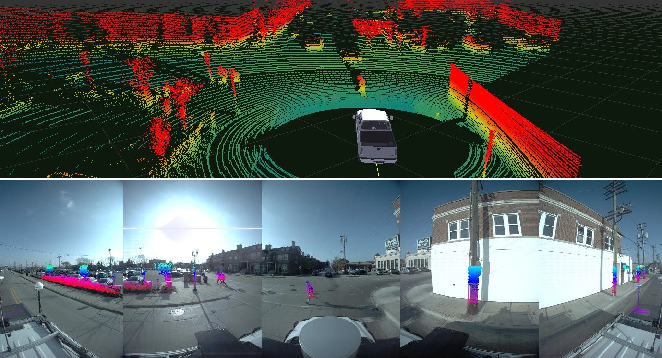
\includegraphics[scale=0.55]{figures/lidar-camera}
\caption[Lidar \& Camera view in self-driving cars]{Same environment, different modes (top: LIDAR view, bottom: camera view)}	
\label{fig:lidar-camera}
\end{figure}


%----------------------------------------------------------------------------------------
%	SECTION 
%----------------------------------------------------------------------------------------

\section{Proposed solution}\label{sec:proposed-solution}
The attention module EMMA is inserted in front of the model, focusing its attention on the modes such that the most useful information passes through while the perturbations are filtered out. The amount of attention distributed to a mode is based on its importance, encompassing three intrinsically tied properties:
\begin{itemize}
\item \textit{relevance}: the quantitative influence of the mode over the predictions
\item \textit{failure intensity}: a measure proportional to the outlyingness\footnote{The outlyingness of a data point tells us how far the observation lies from the center of the training set distribution} of the mode
\item \textit{coupling}: how does the information carried by the mode relate to the other modes? Is it redundant, complementary or conflicting?
\end{itemize}
Let us emphasize that determining the importance is sample dependent, and is thus not easily solved by learning the global tendency.
\begin{figure}[!h]
\centering
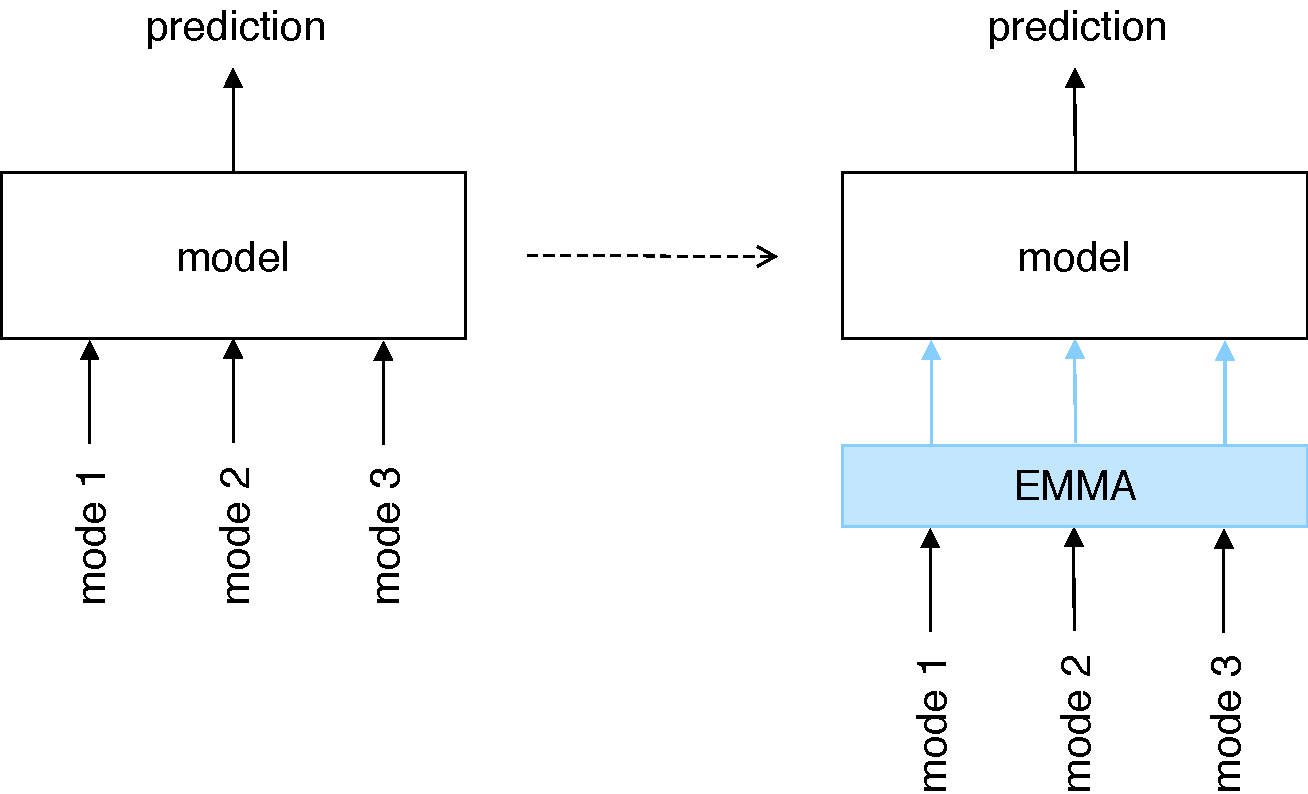
\includegraphics[scale=0.45]{figures/introduction-three-modes-with-emma}
\caption[Multi-Modal model with/without EMMA]{A multi-modal model with three input modes, without EMMA (left), improved with EMMA (right)}	
\label{fig:main-idea}
\end{figure}

\subsection*{Software Implementation}
All the implemented models and experiments are available at this \href{https://github.com/Werenne/energy-based-multimodal-attention}{repository}\footnote{\url{https://github.com/Werenne/energy-based-multimodal-attention}}, with a wiki explaining how to run the experiments; \href{https://pytorch.org/}{PyTorch}\footnote{\url{https://pytorch.org/}} was the main framework used regarding the Machine Learning part.

%----------------------------------------------------------------------------------------
%	SECTION 
%----------------------------------------------------------------------------------------

\section{Contributions}
The work presented in this Master thesis has led to three novel contributions.
\begin{description}
\item \textbf{Contribution 1: an attention module improving significantly the robustness against failing modes.} In Chapter \ref{chapter-emma}, we discuss the design of a new attention mechanism based on energy models \citep{ebm-tutorial}, that can be added to any multi-modal model. 
\item \textbf{Contribution 2: a simple yet powerful regularizer on attention mechanisms.} We slightly modify a common attention function permitting us to establish a link to the concept of capacity in psychology \citep{attention-is-effort}; Capacity is the amount of attention distributed among the inputs. Subsequently, a new regularizer is introduced to control the capacity, which we claim can help generalize against unexpected situations.
\item \textbf{Contribution 3: a unified model for multi-modal attention.} In Chapter \ref{chapter-literature-review}, a review of the literature on attention in humans helps us identify how to construct a more complete multi-modal attention module.
\end{description}

%----------------------------------------------------------------------------------------
%	SECTION 
%----------------------------------------------------------------------------------------

\section{Thesis Outline}
The remainder of this work is organised as follows.
\begin{description}
\item \textbf{Chapter 2} explains the background (i.e. deep learning and energy models) this work is based upon.
\item \textbf{Chapter 3} reviews the literature about attention in psychology and deep learning, and the similarities between them.
\item \textbf{Chapter 4} describes a method for the estimation of the failure intensity of a mode.
\item \textbf{Chapter 5} presents the ideas and architecture of the Energy-based Multi-Modal Attention module (Contribution 1 \& 2).
\item \textbf{Chapter 6} presents a thorough evaluation and analysis of the module outlined in Chapter \ref{chapter-emma}.
\item \textbf{Chapter 7} proposes a unified multi-modal attention module (Contribution 3).
\item \textbf{Chapter 8} concludes this work and suggests possible directions for future research.
\end{description}
\chapter{Background} 
\label{chapter-background} 

%----------------------------------------------------------------------------------------
%	SECTION 
%----------------------------------------------------------------------------------------

\section{Machine Learning}
Machine Learning is a subfield of Artificial Intelligence (see Figure \ref{fig:venn-diagram}) concerned with the design of algorithms that allow machines (e.g. computers, robots, embedded systems) to learn. For a task \textbf{T}, a performance measure \textbf{P} and an amount of data \textbf{D}, the system is said to be learning if it improves its performance \textbf{P} at the task \textbf{T} by increasing \textbf{D} (gain experience). Moreover, there are three main types of learning paradigms, namely supervised, unsupervised and reinforcement learning. In supervised learning \citep{supervised}, the model learns on a labeled dataset, providing an answer that the algorithm can use to evaluate its accuracy on training data. An unsupervised model \citep{unsupervised}, on the contrary, extracts features and patterns from unlabelled data. Lastly, reinforcement learning \citep{sutton} is typically used to train agents in dynamic environments, where the agent is able to act upon the environment. Reinforcement learning is best explained by an analogy. The learning algorithm is like a dog trainer, which teaches the dog (agent) how to respond to specific signs, like a whistle for example. Whenever the dog responds correctly, the trainer gives a reward to the dog, reinforcing the correct behaviour of the dog. Based on these three paradigms, several families of algorithms have been invented. Deep learning \citep{deeplearning-overview} is one of those families and is particularly powerful on perception tasks.
\begin{figure}[!ht]
\centering
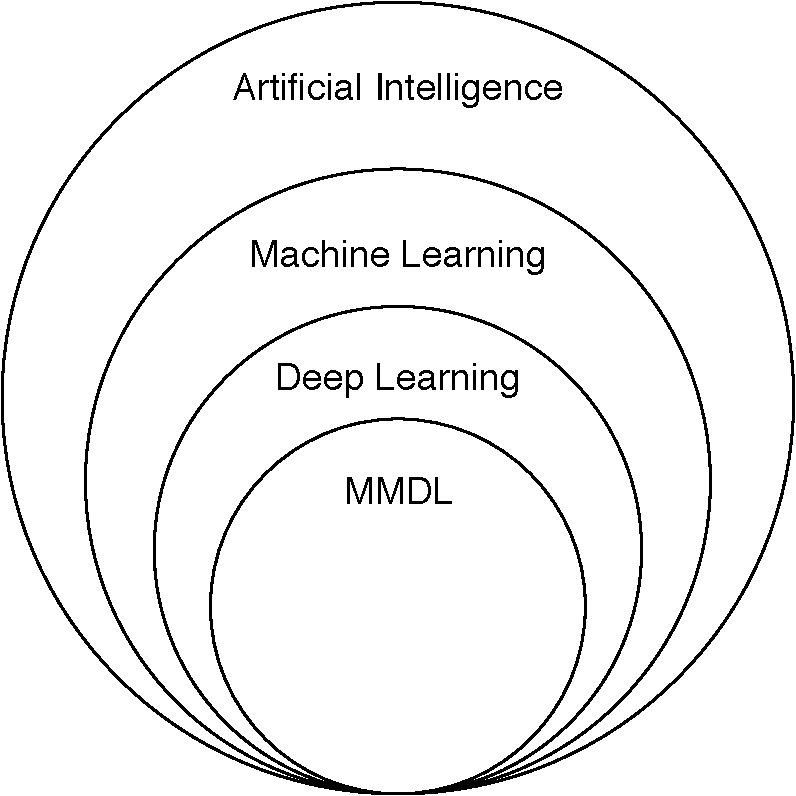
\includegraphics[scale=0.45]{figures/venn}
\caption{Venn diagram of the Artificial Intelligence field.}	
\label{fig:venn-diagram}
\end{figure}


%-----------------------------------
%	SUBSECTION 
%-----------------------------------
\section{Deep Learning}\label{sec:deep-learning}
Deep learning models, also called Deep Neural Networks, offer the significant advantage of being able to learn their own feature representation for the completion of a given task. A neural network is loosely inspired from our own brains, but can best be seen as a series of stacked non-linear parametric functions, enabling the network to learn multiple levels of representation with increasing abstraction. The parameters are tuned by optimizing a loss function with Stochastic Gradient Descent (SGD) or one of its many enhancements \citep{optim-algos}. Let $\bm{\theta}$ be the set of parameters, $\mathcal{L}$ the loss function, $y$ the groundtruth (labels) and $\hat{y}$ the predictions. First, the SGD algorithm estimates the gradient of the cost function on a randomly sampled batch of size $N$ as
\begin{equation}
\mathbf{g} = \frac{1}{N}\nabla_{\bm{\theta}}\sum_{i=1}^N\mathcal{L}(\hat{y}^{(i)},y^{(i)})
\end{equation}
where the computation of the gradient itself is done using back-propagation (BP) \citep{backprop}. The SGD algorithm then follows the estimated gradient downhill, $\bm{\theta} \leftarrow \bm{\theta} - \epsilon\mathbf{g}$ where $\epsilon$ is the learning rate, in the hope of minimizing the loss.

Optimizing the parameters to represent all valid inputs of a task, where the data is often very high-dimensional (e.g., images, sounds, text), may seem hopeless. However, neural networks surmount this obstacle by assuming that these high-dimensional data are lying along low-dimensional manifolds\footnote{A manifold designates a connected set of points that can be approximated well by considering only a small numbers of degrees of freedom.} \citep{goodfellow-book}. An intuitive observation in favour of this claim is that uniform noise essentially never resembles structured inputs from these tasks. More rigorous experiments supporting the manifold hypothesis are \citep{manifold-1, manifold-2, manifold-3}.


\subsection*{Multi-Modal Deep Learning}\label{sec:mmdl}
As a reminder, a modality refers to "the way in which something happened or is experienced" \citep{taxomany-multimodal}. Multi-Modal Deep Learning (MMDL) is simply the research area of neural networks using input samples consisting of multiple modes. Baltrušaitis et al. identified five non-exclusive use-cases of MMDL,
\begin{itemize}
\item \textit{Representation}: learning how to represent and summarize multi-modal data in a way that exploits the complementarity and redundancy
\item \textit{Translation}: learning how to map data from one modality to another (e.g., image captioning)
\item \textit{Alignment}: learning to identify the direct relationships between elements from two or more different modalities (e.g. alignment of sound and video)
\item \textit{Fusion}: learning to join information from two or more modalities to perform predictions 
\item \textit{Co-learning}: learning to transfer knowledge between modalities and their respective predictive models (e.g., zero shot learning)
\end{itemize}
The EMMA module is applied to multi-modal networks performing fusion. Furthermore, networks doing fusion can combine their modalities in three different ways: by early-fusion, late-fusion and an hybrid of the first two. Early-fusion architectures have uni-modal encoders extracting the features of each mode, the obtained features are then concatenated altogether and fed into a common decoder making the predictions (see Figure \ref{fig:early-fusion}). In contrast, late-fusion has uni-modal predictors for each mode, followed by a decoder weighting the uni-modal predictions to compute the final prediction. 
\begin{figure}[!h]
\centering
\begin{subfigure}{.45\textwidth}
\vspace*{15.5mm}
  \centering
  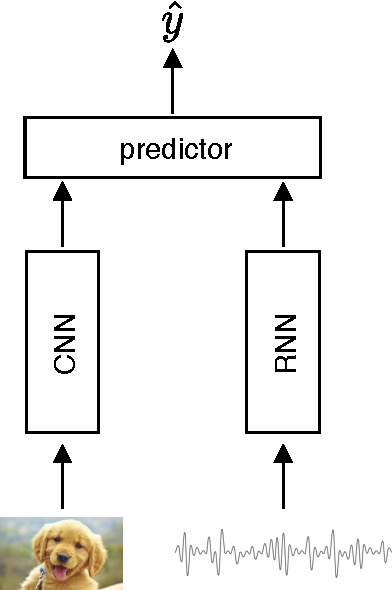
\includegraphics[width=.55\linewidth]{figures/early-fusion}
  \vspace*{3mm}
  \caption{Early-fusion}
  \label{fig:early-fusion}
\end{subfigure}%
\begin{subfigure}{.45\textwidth}
  \centering
  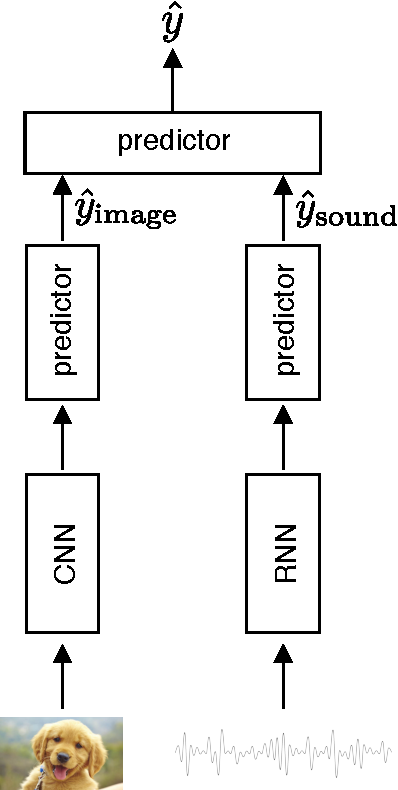
\includegraphics[width=.55\linewidth]{figures/late-fusion}
  \vspace*{2mm}
  \caption{Late-fusion}
  \label{fig:late-fusion}
\end{subfigure}
\caption[Early and late fusion]{Fusion of images and sounds for a classification task with a Convolutional Neural Network (CNN) \citep{image-recognition}, Recurrent Neural Network (RNN) \citep{machine-translation}.}
\label{fig:fusion}
\end{figure}


%----------------------------------------------------------------------------------------
%	SECTION 
%----------------------------------------------------------------------------------------
\section{Physics meets Deep Learning}\label{sec:ebm}
Modelling complex probability distributions by parametric functions such as deep learning models is a difficult task, because all the probabilities must be positive and sum up to one. At its origins, many researchers in deep learning had an academic background in physics, from which they regularly found inspiration to solve problems. An example of this is the distribution of kinetic energies among molecules of gas, called the Boltzmann distribution, and given by
\begin{equation}
p(E_i) = \frac{1}{Z}e^{-E_i/k_B T} \quad \text{with the partition function} \quad Z = \int e^{-E_j/k_B T}
\label{eq:boltzmann-distrib}
\end{equation}
where $E_i$ is the kinetic energy of molecule $i$, $k_B$ the Boltzmann constant and $T$ the temperature of the environment. The first thing to notice is that all the probabilities are positive and sum up to one for any set of combinations of energies $E_i$. Another observation to make is that high values of energies are unlikely ($E_i \propto -\log p(E_i)$), unless the temperature is sufficiently high enough. To sum it up, the Boltzmann distribution can be used to normalize any function to a distribution, where the temperature $T$ is a parameter influencing the entropy of the distribution. The Boltzmann distribution has two major applications in deep learning. First, it corresponds to the soft-max activation function \citep{softmax}, employed commonly for the purpose of outputting probabilities in multi-category classification tasks. Secondly, it was also used by deep learning researchers to construct energy-based models \citep{ebm-tutorial}. These types of neural networks optimize an energy function to be low on the data manifold and high everywhere else (see Figure \ref{fig:ebm-intervals}), which is the mapped to probabilities via the Boltzmann distribution. A few examples of efficient energy-based models are Generative Adversarial Networks (GAN) \citep{gan}, Variational Autoencoders (VAE) \citep{kingma-vae} and Denoising Autoencoders (DAE) \citep{dae-vincent}. The latter will be used in this work to measure the outlyingness of the data (see Chapter \ref{chapter-energy-estimation}).
\begin{figure}[!ht]
\centering
\includegraphics[scale=0.55]{figures/ebm-intervals-t}
\caption[Energy surface evolution]{The shape of the energy surface at four intervals. Along the x-axis is the variable X and along the y-axis is the variable Y . The shape of the surface at (a) the start of the training, (b) after 15 epochs over the training set, (c) after 25 epochs, and (d) after 34 epochs. The energy surface has attained the desired shape: the energies around the training samples are low and energies at all other points are high. \textit{Image and caption from} \,\citep{ebm-tutorial}.}
\label{fig:ebm-intervals}
\end{figure} 
\chapter{Literature Review}\label{chapter-literature-review} 

The purpose of this chapter is to review the state-of-the-art literature of multi-modal attention. The first section describes attention in humans from both a psychological and a neurological point of view. We argue this will give the reader more intuition about attention in deep learning. The second part moves on to the different attention mechanisms in deep learning, in particular self-attention and crossmodal attention. 


%-----------------------------------
%	SECTION 
%-----------------------------------
\section{Attention in Humans}
The most profound effect of attention is its capacity to bring the attended stimuli into the forefront of our conscious experience while unattended stimuli fades into the background, increasing the processing efficiency at every stage of perception \citep{watzl}. A widely held assumption in the psychology literature is that the most fundamental function of attention is selection. But also at the level of single neurons, neuroscientist typically thought of attention in terms of selection between stimuli competing for the same neural receptive field \citep{neuro-level}. Daniel Kahneman, an authorithy in psychology and economy, investigated the way in which humans perform multi-tasking (i.e., solve a multi-modal problem). Kahneman claimed that attention was more than selection, that it could be viewed as a limited resource being shared among the different modes, but he could not generalize his findings to the intra-modal level\footnote{Intra-modal attention manifests itself only in a subset of the mode, whereas inter-modal attention is between modes.}. Moreover, the selection theory has been vigorously challenged in recent years by the amplification theory, where attention is an additional activity that interacts with built-in perceptual mechanisms by amplifying some of the input signals \citep{amplification}. Furthermore, the absolute intensity of amplification is not important, in contrary it is the relative intensity between the inputs that matters (\textit{the contrast effect}). Notice that the amplification theory generalizes the concept of capacity to the intra-modal level and neural level. Interestingly, we will see that the basic principles of attention mechanisms in deep learning has significant similarities with amplification.

Regarding multi-modal attention, three types can be distinguished: endogenous, exogenous and crossmodal attention \citep{crossmodal}. People orient their attention endogenously whenever they voluntarily choose to attend to something, such as when listening to a particular individual at a noisy cocktail party, or when concentrating on the texture of the object that they happen to be holding in their hands. By contrast, exogenous orienting occurs when a person’s attention is captured reflexively by the sudden onset of an unexpected event, such as when a mosquito suddenly lands on our arm. Lastly, crossmodal attention refers to the interaction of attention between two or more modes such as using visual clues (e.g. lip movements) to focus on the voice of a particular individual at a noisy cocktail party.


%-----------------------------------
%	SECTION 
%-----------------------------------
\section{Attention in Deep Learning}
Attention-based approaches in deep learning focus on network architectures that specifically attend to regions of their input space. The most common way to do this, is by multiplying the input by an attention mask, where the attention mask consist of normalized continous values between zero and one. Observe the similarity with the amplication theory described in the previous section. In self-attention \citep{bahdanau}, the attention mask is computed from the same mode on which it is applied. Conversely, for crossmodal attention mechanisms \citep{crossmodal-object-detection}, the attention mask is computed from multiple modes. 

Self-attention was first introduced in natural language processing (NLP) for machine translation tasks by \citep{bahdanau}. It helped the translation task by enabling the model to automatically search for parts of a source sentence that are relevant to predicting the next target work. With this approach, Bahdanau et al. achieved a translation performance comparable to the existing state-of-the-art phrase-based system on the task of English-French translation. Since then it has become a prominent tool in NLP but has also been used in a variety of other tasks such as image classification. \citep{self-capsule} uses self-attention to learn to suppress irrelevant regions in images and highlight salient features useful for the specific classification task. The authors in \citep{self-capsule} reduced the computation load and were able to compensate the absence of a deeper network by using the self-attention, without having a decreased classification performance. For a detailed review on this self-attention mechanisms, see \citep{attention-review}.

In \citep{looking-to-listen}, an audio-visual model is presented for isolating a single speech signal form a mixture of sounds such as other speakers and background noise (see Figure \ref{fig:looking-to-listen}). Crossmodal attention is used to focus on certain parts of the audio with respect to an image of the desired speaker. The authors showed superior results compared to state-of-the-art audio-only methods. Similar works \citep{cross-transformer, crossmodal-object-detection, crossmodal-video-caption} are using crossmodal attention and have attained impressive results. However, most research using crossmodal attention has tended to focus on obtaining better predictions rather than improving the robustness. A few exceptions are discussed below.
\begin{figure}[!ht]
\centering
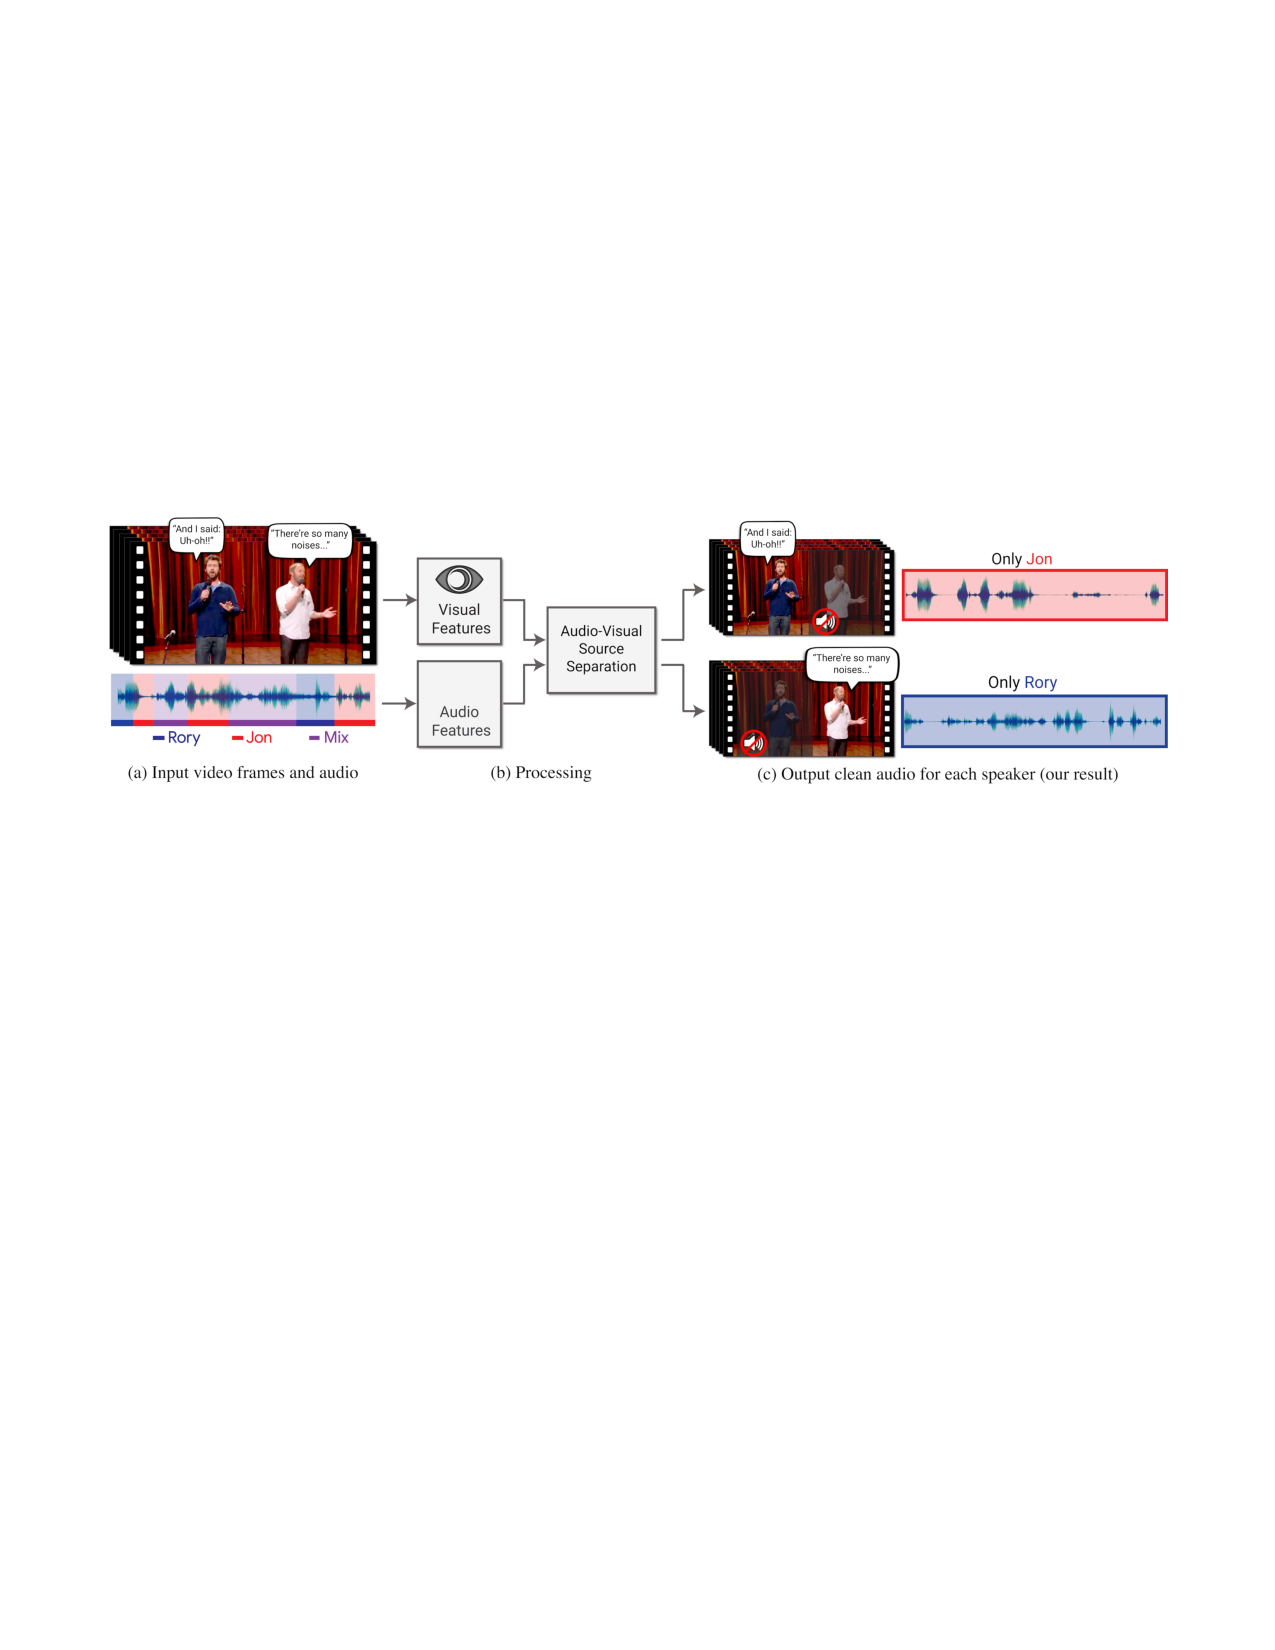
\includegraphics[scale=0.85]{figures/look-to-listen}
\caption[Looking to Listen framework]{The authors of \citep{looking-to-listen} present a model for isolating and enhancing the speech of desired speakers in a video. (a) The input is a video (frames + audio track) with one or more people speaking, where the speech of interest is interfered by other speakers and/or background noise. (b) Both audio and visual features are extracted and fed into a joint audio-visual speech separation model. The output is a decomposition of the input audio track into clean speech tracks, one for each person detected in the video (c). This allows them to then compose videos where speech of specific people is enhanced while all other sound is suppressed. Their model was trained using thousands of hours of video segments from our new dataset, AVSpeech. The “Stand-Up” video (a) is courtesy of Team Coco. \textit{Image and caption from} \citep{looking-to-listen}}
\label{fig:looking-to-listen}
\end{figure}

A work investigating how multimodal fusion can help against failing modes is \citep{afouras}. Their model fuses audio and video to obtain better speech-to-text. Interestingly, Afouras et al. use a combination of self-attention mechanisms followed by a crossmodal attention layer. The model was tested on thousands of natural sentences of British television. Furthermore, they added babble noise with 0dB signal-to-noise ratio to the audio streams, where the babble noise samples are synthesized by mixing the signals of 20 different audio samples from the dataset. The audio-visual model achieved a 13.7\% word error rate (WER) on the dataset without noise, and a 33.5\% WER on the dataset with noise whereas the audio-only model only achieved 64.7\% WER. Despite obtaining great results, a major weakness with this experiment, however, is that their test set is corrupted in the exact same manner as their training set; there are also no varying levels of noise between the two modes. Additionally, the attention module is not constructed to detect unseen samples. To sum it up, the model was not tested against realistic failing modes situations.

The work that is most relevant to our proposed method is the attentive context proposed in \citep{audiovisual-attention}, which also incorporates attention on the inter-modal level to filter the perturbations (see Figure \ref{fig:noise-tolerant}). The model is evaluated on a face-verification task, receiving a voice and a face. The attention mask $[\alpha_v,\alpha_f]$ is computed via a linear function, $f_{\text{att}} = \mathbf{W}^T[\mathbf{e}_v, \mathbf{e}_f] + \mathbf{b}$, on the embeddings $\mathbf{e}_v$ and $\mathbf{e}_f$. Several defects of the attention function $f_{\text{att}}$ can be observed: 
\begin{enumerate}
\item The function is likely to be to simple to neither capture complicated dependencies between the modes, nor to recognize unseen data.
\item The way in which the function is designed forces the model to extract embeddings of the same size, which may be a significant constraint when combining modes from low and high-dimensional data.
\item TODO: explain no control (capacity, temperature)
\end{enumerate}

\begin{figure}[!ht]
\centering
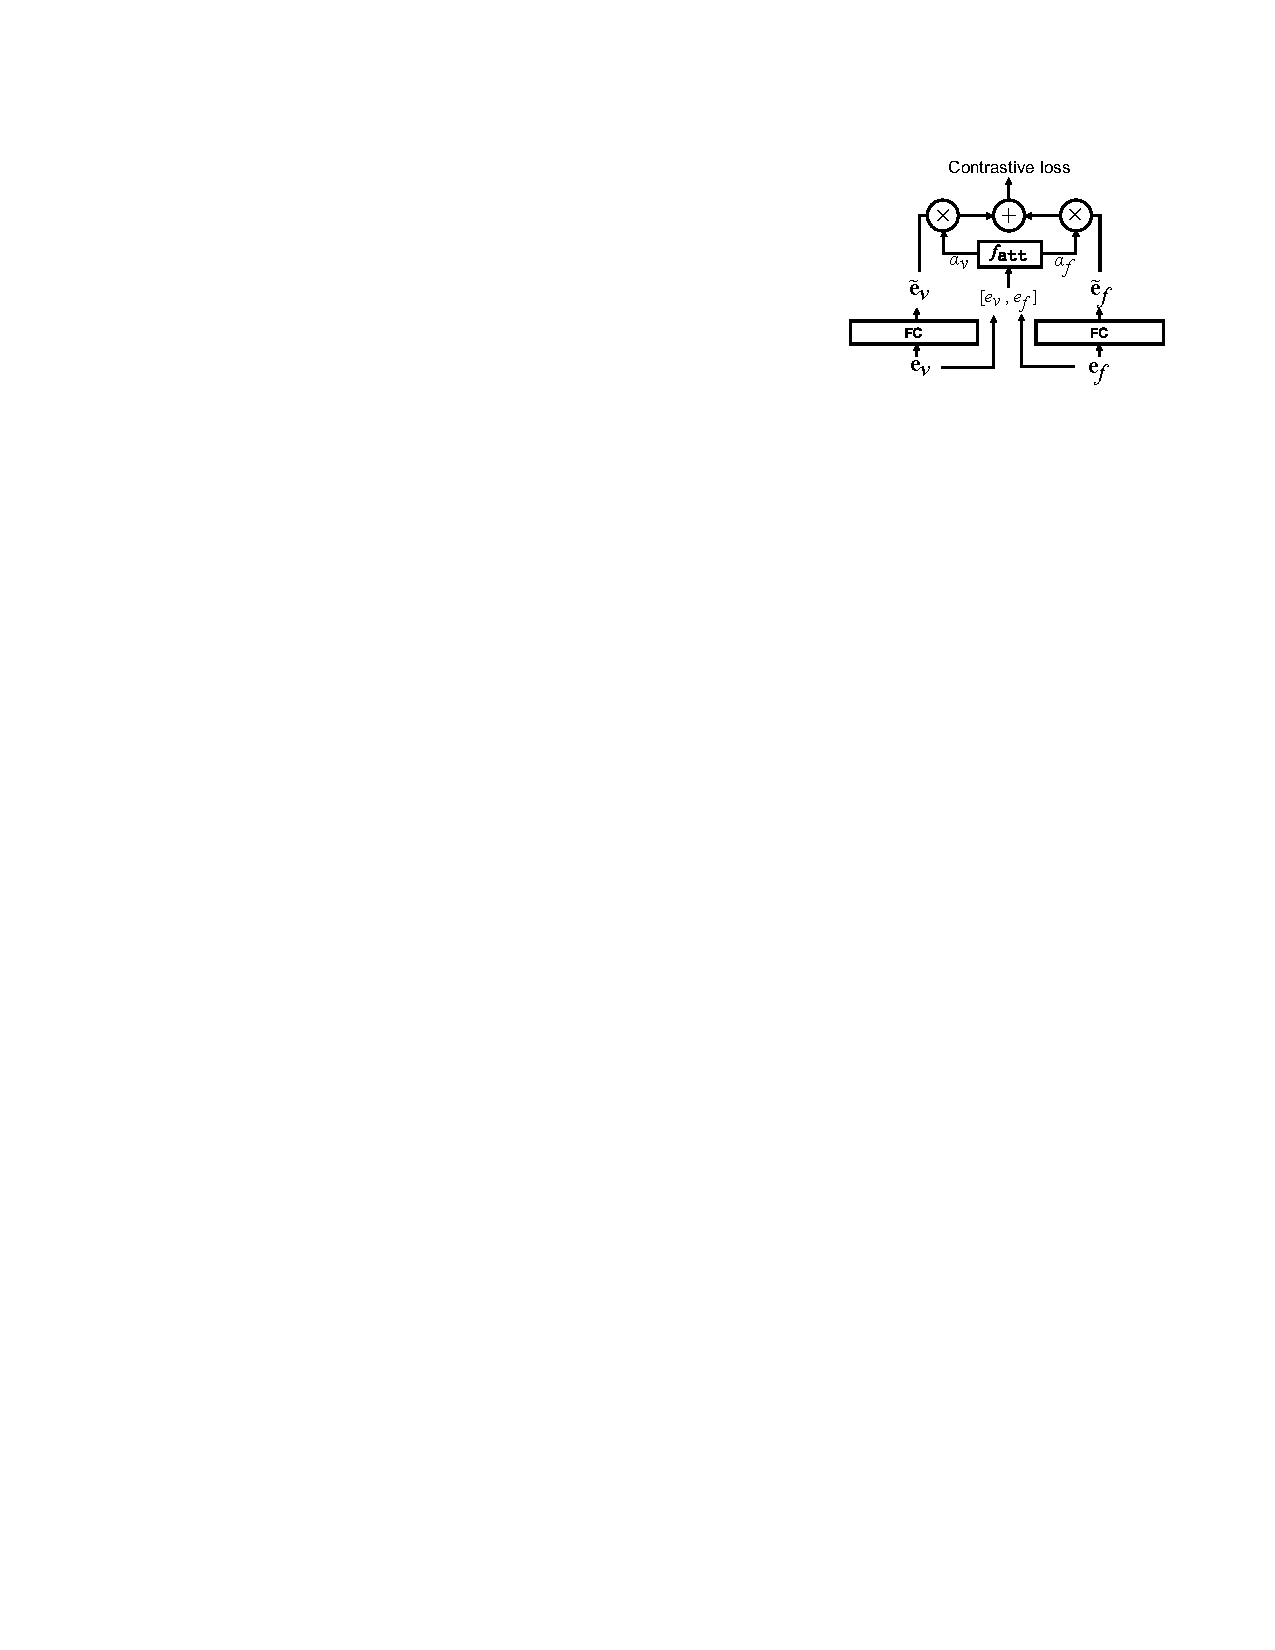
\includegraphics[scale=0.85]{figures/noise-tolerant}
\caption[Noise-tolerant fusion model]{Neural network based fusion approaches. $\mathbf{e}_v$ : speaker embedding, $\mathbf{e}_f$ : face embedding. FC denotes a fully connected layer. \textit{Image from} \citep{audiovisual-attention}}
\label{fig:noise-tolerant}
\end{figure}




\chapter{Energy Estimation} 
\label{chapter-energy-estimation} 

In the introduction we suggested that a mode of the input sample that is significantly different from the training distribution may cause undesired activations in the neural network, i.e. the failure intensity of a mode is correlated with its likelihood relative to the training distribution. Furthermore, in Section \ref{sec:ebm} we explained that the energy function in energy-based models is proportional to the negative log-likelihood (NLL), which could thus be used to evaluate the failure intensity of a mode. This chapter discusses how to derive the energy function of a denoising autoencoder, which will be used as a metric for the failure intensity (discussed in Chapter \ref{chapter-introduction}).

%----------------------------------------------------------------------------------------
%	SECTION 
%----------------------------------------------------------------------------------------

\section{Autoencoders}

Autoencoders (AE) are models trained to reproduce their inputs to their outputs. An autoencoder is composed of two main parts, the encoder $f$ and the decoder $g$. The input $\mathbf{x} \in  \mathbb{R}^L$ is passed through the encoder $f: \mathbb{R}^L \mapsto \mathbb{R}^U$ as $f(\mathbf{x}) = h(W_f\mathbf{x} + \mathbf{b}_f) = \mathbf{u}$, where $h(\cdot)$ is an activation function applied element-wise and $ \mathbf{u}$ represents the hidden layer. The decoder $g: \mathbb{R}^U \mapsto \mathbb{R}^L$ is then in charge of reconstructing the input, $g(\mathbf{u}) = W_g\mathbf{u} + \mathbf{b}_g$. The output is often called the reconstruction and is written  $r(\mathbf{x}) = g(f(\mathbf{x}))$ with $r: \mathbb{R}^L \mapsto \mathbb{R}^L$. Autoencoders are trained in an unsupervised manner, most of the time using the mean-squared error between input and output as a loss function, $\mathcal{L}_{\text{MSE}} = \lVert r(\mathbf{x}) - \mathbf{x} \rVert_2^2$. Training a model to copy its input may seem useless. To answer this point, we need to distinguish two families of autoencoders, namely undercomplete and overcomplete autoencoders.

\begin{figure}[!h]
\centering
\begin{subfigure}{.5\textwidth}
\vspace*{12mm}
  \centering
  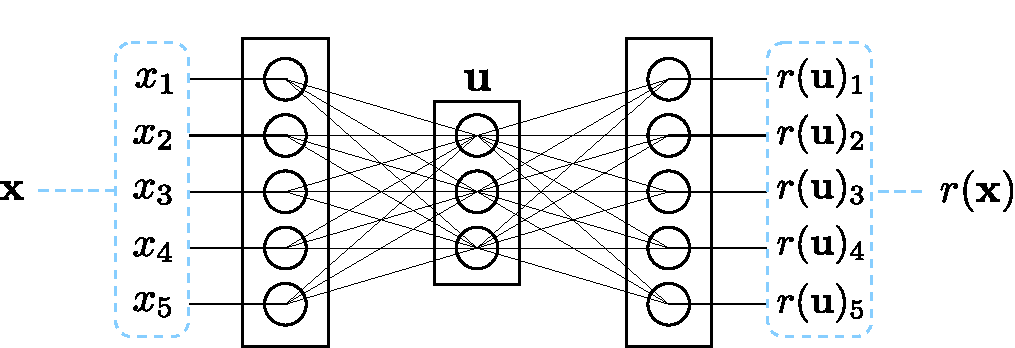
\includegraphics[width=.95\linewidth]{figures/autoencoder-undercomplete}
  \vspace*{8mm}
  \caption{Undercomplete AE}
  \label{fig:undercomplete-ae}
\end{subfigure}%
\begin{subfigure}{.5\textwidth}
  \centering
  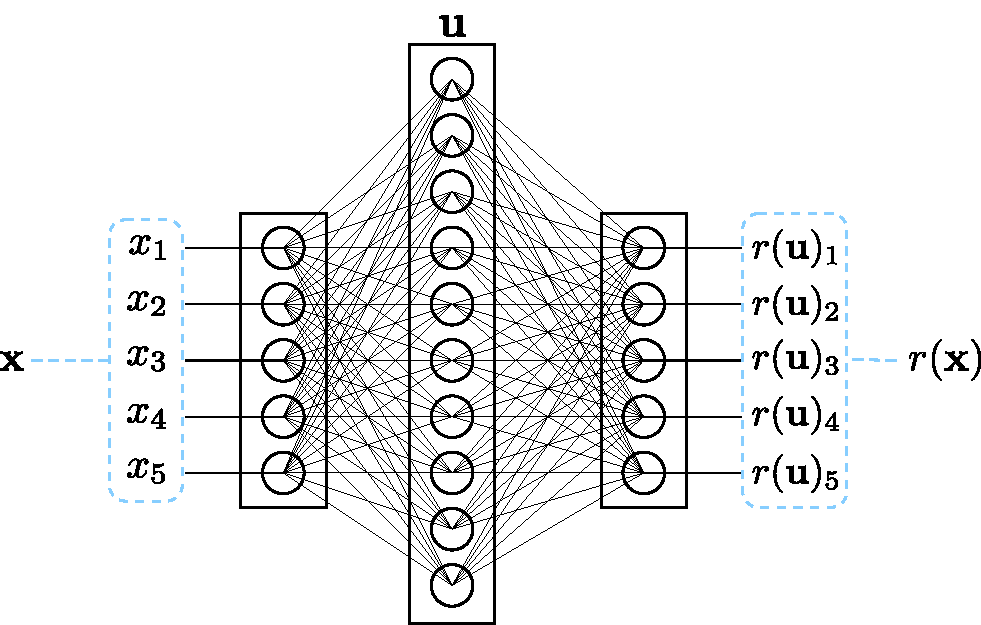
\includegraphics[width=.95\linewidth]{figures/autoencoder-overcomplete}
  \caption{Overcomplete AE}
  \label{fig:overcomplete-ae}
\end{subfigure}
\caption{The architecture of the two families of autoencoders}
\label{fig:under-over-ae}
\end{figure}

%-----------------------------------
%	SUBSECTION 
%-----------------------------------
\subsection*{Undercomplete autoencoders}
An autoencoder is said to be undercomplete when the size of the hidden layer $\mathbf{u}$ is smaller than the size of the input/output layers, i.e. $U < L$ (see Figure \ref{fig:undercomplete-ae}). This amounts to constructing a low-dimensional representation of the input, and information is therefore lost in the process. It can be thought of as a non-linear principal component analysis \citep{pca-ae-1, pca-ae-2} as the values formed in the hidden layer are a non-linear representation in latent space of the input. As can be seen in Figure \ref{fig:reconstruction}, minimizing the mean squared error is similar to minimizing the Euclidean norm of the vector $r(\mathbf{x}) - \mathbf{x}$.
\begin{figure}[!h]
\centering
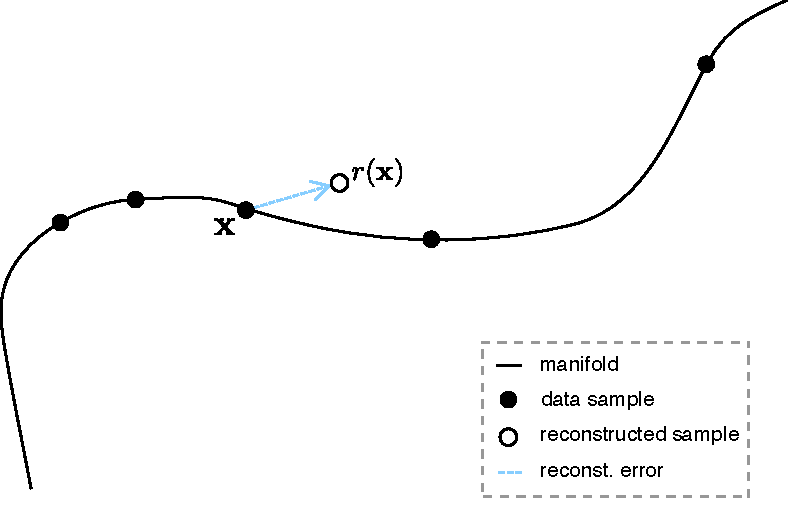
\includegraphics[scale=0.55]{figures/reconstruction}
\caption[Vectorial representation of undercomplete AE]{Vectorial representation of an undercomplete reconstruction process.}
\label{fig:reconstruction}
\end{figure}

%-----------------------------------
%	SUBSECTION 
%-----------------------------------
\subsection*{Overcomplete autoencoders}\label{sec:overcomplete}
Conversely, an overcomplete AE has more hidden units than its input/output layer, i.e. $U > L$ (see Figure \ref{fig:overcomplete-ae}). Hence, the model could thus learn to perfectly copy its input through the $U$ hidden units and reproduce it at the output. However, the input is corrupted before being passed through the encoder, whereas the decoder is forced to reconstruct the original input, i.e. the model learns to denoise signals. This type of AE is called a denoising autoencoder (DAE). More formally, the input is corrupted with some small isotropic noise $\tilde{\mathbf{x}} = \mathbf{x} + \mathbf{\epsilon}$ where $\epsilon \sim \mathcal{N}(0,\,\sigma^{2})$, with the training loss 
\begin{equation}
\mathcal{L}_{\text{MSE}} = \lVert r(\tilde{\mathbf{x}}) - \mathbf{x} \rVert_2^2
\end{equation}
It is worth noticing the difference with the loss function of the undercomplete AE. We verify in Figure \ref{fig:reconstruction-dae} that minimizing the loss implies that the \textit{reconstruction error} $r(\tilde{\mathbf{x}}) - \tilde{\mathbf{x}}$ will converge to $-(\tilde{\mathbf{x}} - \mathbf{x})$ i.e. the model learns to invert the corruption process.

\begin{figure}[!h]
\centering
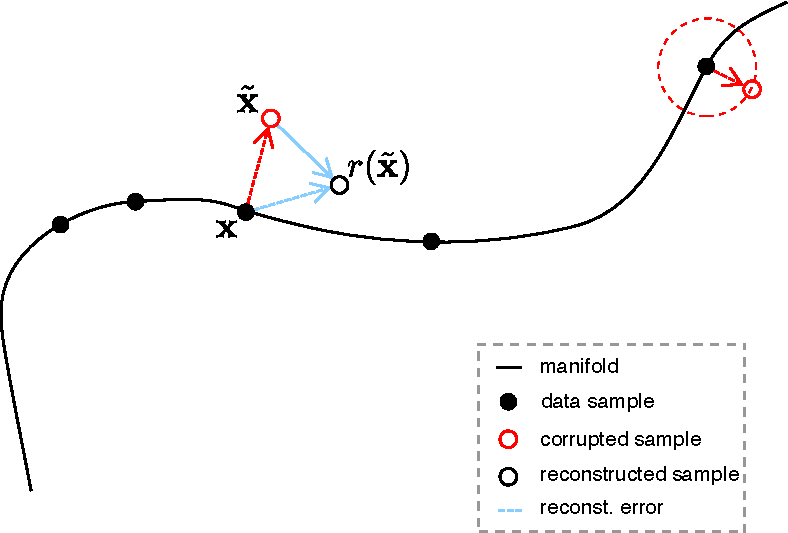
\includegraphics[scale=0.55]{figures/reconstruction-denoising}
\caption[Vectorial representation of overcomplete AE]{Vectorial representation of an overcomplete reconstruction process.}
\label{fig:reconstruction-dae}
\end{figure}

%----------------------------------------------------------------------------------------
%	SECTION 
%----------------------------------------------------------------------------------------

\section{Energy in Autoencoders}

The authors in \citep{alainbengio} found that the reconstruction error of a trained denoising autoencoder is proportional to the score (gradient of log-likelihood)
\begin{equation}
r(\tilde{\mathbf{x}}) - \tilde{\mathbf{x}} \propto \frac{\partial \log p(\tilde{\mathbf{x}})}{\partial \tilde{\mathbf{x}}} 
\label{eq:score-reconstruction}
\end{equation} 
To put it differently, the reconstruction error points towards the corresponding most likely datapoint. This result is not particularly suprising, as denoising a signal is essentially equivalent to finding the most likely datapoint among nearby samples in the distribution (see Figure \ref{fig:reconstruction-dae}). To illustrate Equation (\ref{eq:score-reconstruction}), we train a DAE on a generated circle manifold (more details about this experiment in Section \ref{sec:experiment-I}). As we can see below, the vector field of the reconstruction error does indeed point towards the data manifold\footnote{We refer broadly to a data manifold as a connected set of points that can be approximated well by considering only a small numbers of degrees of freedom.}.
\begin{figure}[!h]
\centering
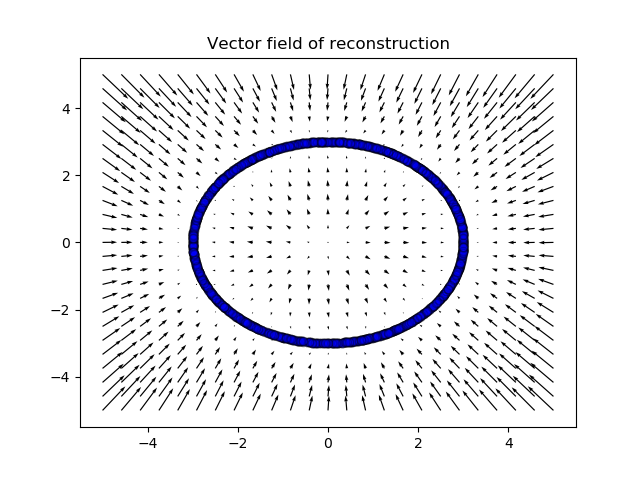
\includegraphics[scale=0.6]{figures/circle-vector-field}
\caption[Vector field circle manifold]{Vector field of reconstruction error on circle manifold. No corruption is applied at test time, the reconstruction error vector is simply the output minus the input. The experimental setup is described in Section \ref{sec:experiment-I}.}
\label{fig:vf-circle}
\end{figure}
Alternatively, Figure \ref{fig:vf-circle} may be interpreted in terms of forces deriving from potential fields as observed in physics. This interpretation can be useful to distinguish the manifold since it acts as a sink in the vector field i.e., has a low potential energy. 

A vector field is the gradient of a potential energy field if it satisfies a simple condition called the integrability criterion\footnote{See Appendix \ref{sec:criterion}}. In \citep{potentialenergy}, the authors found that using tied weights ($W_f = W_g^T = W$), produces an autoencoder configuration whose reconstruction error field satisfies the aforementioned integrability criterion. Indeed, one successively finds
\begin{equation}
\begin{split}
\frac{\partial(r(\tilde{\mathbf{x}})_i- \tilde{x}_i)}{\partial  \tilde{x}_j} &= \frac{\partial\big[W^T h(W\tilde{\mathbf{x}} + \mathbf{b}_f) + \mathbf{b}_g\big]_i}{\partial  \tilde{x}_j} - \frac{\partial\tilde{x}_i}{\partial  \tilde{x}_j} \\
&= \sum_k W_{ik} \frac{\partial h(W\tilde{\mathbf{x}} + \mathbf{b}_f)}{\partial(W\tilde{\mathbf{x}} + \mathbf{b}_f)}W_{jk} - \delta_{ij}   \\
&= \frac{\partial(r(\tilde{\mathbf{x}})_j- \tilde{x}_j)}{\partial  \tilde{x}_i}
\end{split}
\end{equation} 
where $\delta_{ij}$ denotes the Kronecker delta. Hence, under this assumption, the reconstruction error can be expressed as the gradient of a scalar field, the potential energy $-\Psi$, such that $r(\tilde{\mathbf{x}}) - \tilde{\mathbf{x}} = -\partial \Psi(\tilde{\mathbf{x}})/\partial \tilde{\mathbf{x}}$. Thereupon, the reconstruction process can be seen as a gradient descent in the potential energy space \citep{potentialenergy}. A key insight to gain from these developments and Equation (\ref{eq:score-reconstruction}) is that the aforementioned potential energy is in fact proportional to the NLL,
\begin{equation}
\frac{\partial \Psi(\tilde{\mathbf{x}})}{\partial \tilde{\mathbf{x}}} \propto -\frac{\partial \log p(\tilde{\mathbf{x}})}{\partial \tilde{\mathbf{x}}} \Rightarrow  \Psi \propto -\log p
\end{equation}
Since the gradient of the potential energy can be expressed in terms of the reconstruction error, the potential energy $\Psi$ can be computed by integrating the latter,
\begin{equation}
 \Psi(\tilde{\mathbf{x}}) = -\int (r(\tilde{\mathbf{x}}) - \tilde{\mathbf{x}})d\tilde{\mathbf{x}} 
 \label{eq:psi-int}
\end{equation}
Now, expressing $r$ in terms of $f = h(W\mathbf{x} + \mathbf{b}_f)$ and $g = W^Tf(\mathbf{x}) + \mathbf{b}_g$ in (\ref{eq:psi-int}), and following the developments made in \citep{potentialenergy}, we obtain
\begin{equation}
\Psi(\tilde{\mathbf{x}})= -\int f(\tilde{\mathbf{x}})d\tilde{\mathbf{x}} + \frac{1}{2} \lVert \tilde{\mathbf{x}} + \textbf{b}_g \rVert_2^2 + \text{const}
\end{equation} 
In this work only the sigmoid will be used as an activation function $h$, so that the expression of $f$ can be written explicitly and
\newcommand\boxedB[1]{{\setlength\fboxsep{8pt}\boxed{#1}}}
\begin{equation}
\boxedB{\Psi(\tilde{\mathbf{x}}) =  -\sum_k \log(1 + \text{exp}(W_{.k}^T \tilde{\mathbf{x}} + b_k^f)) + \frac{1}{2} \lVert \tilde{\mathbf{x}} - \textbf{b}_g \rVert_2^2 + \cancel{\text{const}} \propto -\log p(\tilde{\mathbf{x}})}
\label{eq:potential-prop}
\end{equation}
where $W_{.k}^T$ is the $k^{\text{th}}$ column of $W^T$, and $b_k^f$ the $k^{\text{th}}$ entry of $\textbf{b}_f$. All intermediate steps between (\ref{eq:psi-int}) and (\ref{eq:potential-prop}) are detailed in \citep{potentialenergy}. It is worth remarking that the potential energy can be negative by construction. 

%----------------------------------------------------------------------------------------
%	SECTION 
%----------------------------------------------------------------------------------------

\section{Experiment I}\label{sec:experiment-I}
In this experiment, two simple data manifolds are generated, on which separate denoising autoencoders are trained. In order to evaluate the suitability of the potential energy as a proxy for the NLL, the former is plotted on a grid for each of these autoencoders.. As a comparison, we also compute the reconstruction error, $\lVert r(\tilde{\mathbf{x}}) - \tilde{\mathbf{x}} \rVert_2^2$, which is sometimes used in the Machine Learning community as a way to detect outliers. 
\subsection*{Manifolds}
The manifolds maps a set of N scalar values $\{t_1, \ldots, t_N\}$ drawn uniformly at random in $[0, 2\pi]$ into a set of vectors $\{\mathbf{x}^1, \ldots, \mathbf{x}^N\} \subset \mathbb{R}^2$. The entries of these vectors are obtained as
$$
\text{wave}  \begin{cases}
      x_1^k = t_k - \pi \\
      x_2^k = \sin(t_k)
    \end{cases}  \qquad \text{circle}  \begin{cases}
     x_1^k = 3\sin(t_k) \\
      x_2^k = 3\cos(t_k)
    \end{cases}
$$
The resulting structures are illustrated in Figure \ref{fig:generate-manifold}.
\begin{figure}[!h]
\centering
\begin{subfigure}{.5\textwidth}
  \centering
  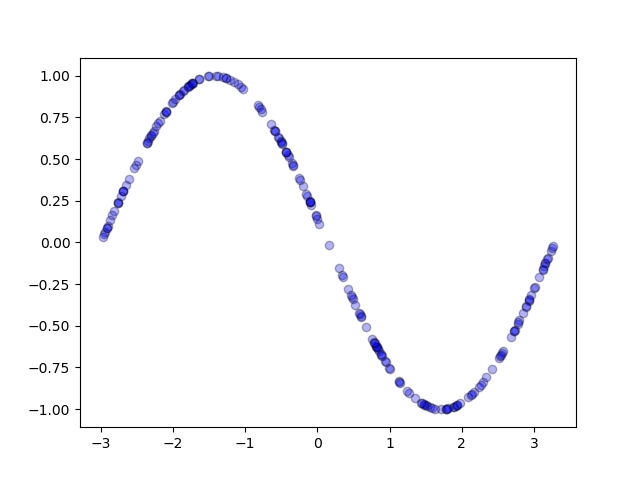
\includegraphics[width=.95\linewidth]{figures/wave-manifold}
  \caption{Wave}
\end{subfigure}%
\begin{subfigure}{.5\textwidth}
  \centering
  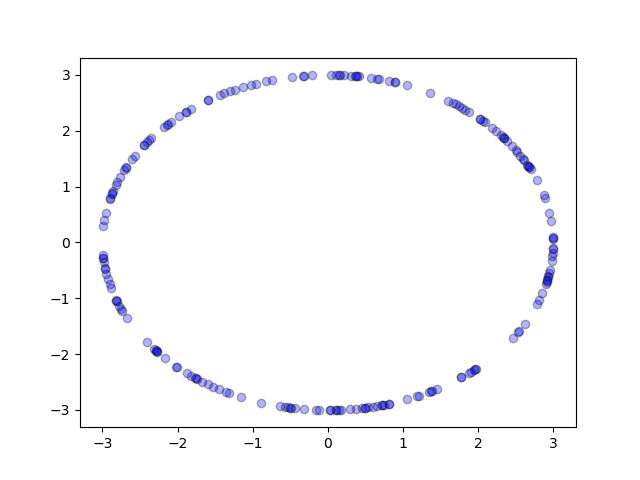
\includegraphics[width=.95\linewidth]{figures/circle-manifold}
  \caption{Circle}
\end{subfigure}
\caption{Manifold generation with 200 samples.}
\label{fig:generate-manifold}
\end{figure}

\subsection*{Setup}
Each autoencoder has 8 hidden units, is trained for 25 epochs, with a batch size of 100, a corruption noise $\sigma = 0.008$ and a learning rate of $1e^{-3}$. The optimizer used is \textit{Adam} \citep{kingma}.

\subsection*{Results}
As expected the vector fields of the reconstruction errors are directed towards the manifolds (see Figure \ref{fig:exp1-vector-fields}), the manifolds acting as sinks. Notably, observe the presence of a source at the origin for the circle manifold (see Figure \ref{fig:exp1-vf-circle}).
\begin{figure}[!h]
\centering
\begin{subfigure}{.5\textwidth}
  \centering
  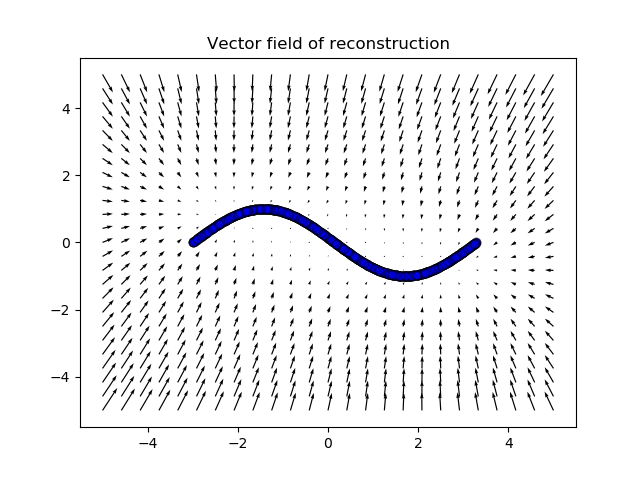
\includegraphics[width=.95\linewidth]{figures/wave-vector-field}
  \caption{Wave}
\end{subfigure}%
\begin{subfigure}{.5\textwidth}
  \centering
  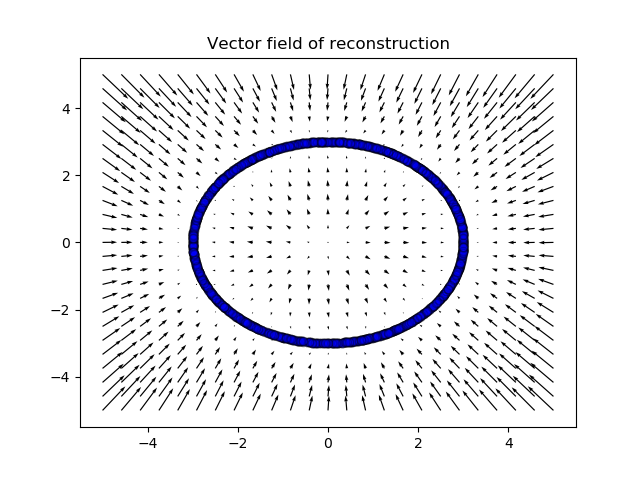
\includegraphics[width=.95\linewidth]{figures/circle-vector-field}
  \caption{Circle}
  \label{fig:exp1-vf-circle}
\end{subfigure}
\caption[Vector fields on wave and circle manifold]{Vector fields of the reconstruction error evaluated on a mesh grid.}
\label{fig:exp1-vector-fields}
\end{figure}

The energy function and the norm of the reconstruction error are computed and plotted onto heatmaps (see Figure \ref{fig:exp1-heatmaps}). We can see that the two estimators have low values in the neighbourhood of the manifold and are high everywhere else. However, the norm of the reconstruction error has also low values at the origin, due to the source in its vector field. This issue makes it difficult in general to use it as a robust criterion to detect and quantify out-of-distribution samples.
\begin{figure}[!h]
\centering
\begin{subfigure}{.5\textwidth}
  \centering
  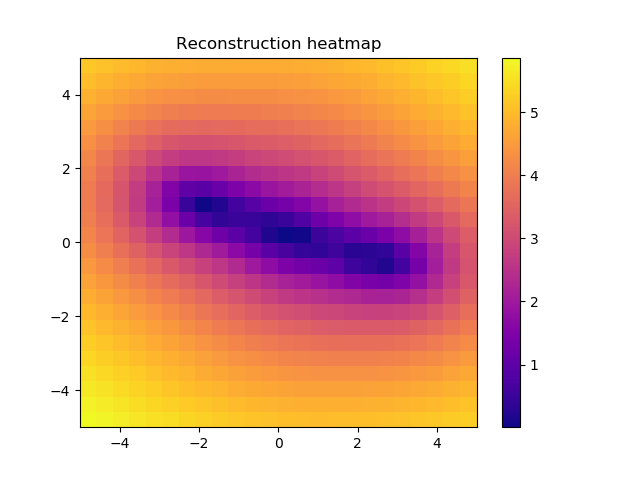
\includegraphics[width=.95\linewidth]{figures/wave-quantifier-reconstruction}
  \caption{Wave - Norm reconstruction error}
\end{subfigure}%
\begin{subfigure}{.5\textwidth}
  \centering
  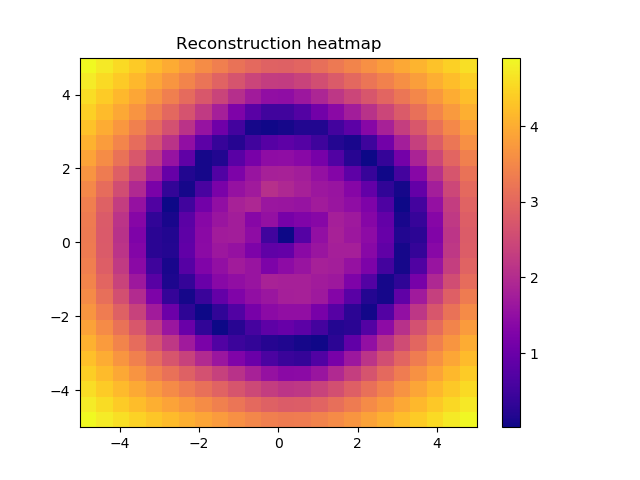
\includegraphics[width=.95\linewidth]{figures/circle-quantifier-reconstruction}
  \caption{Circle - Norm reconstruction error}
\end{subfigure}
\begin{subfigure}{.5\textwidth}
  \centering
  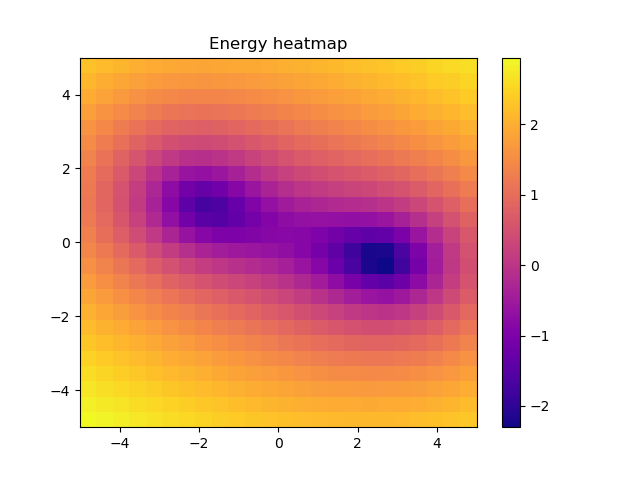
\includegraphics[width=.95\linewidth]{figures/wave-quantifier-energy}
  \caption{Wave - Potential energy}
\end{subfigure}%
\begin{subfigure}{.5\textwidth}
  \centering
  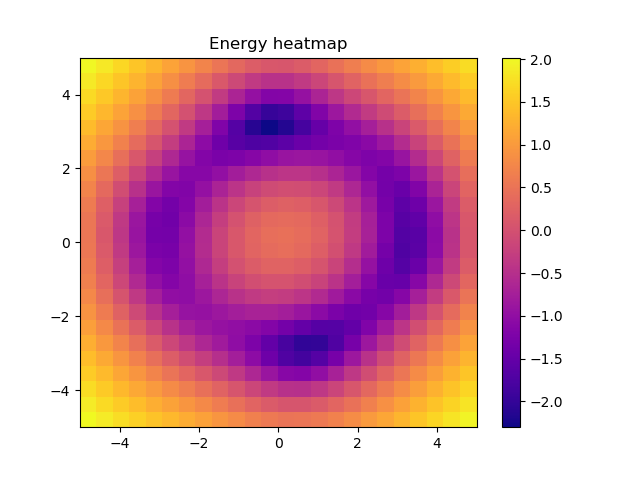
\includegraphics[width=.95\linewidth]{figures/circle-quantifier-energy}
  \caption{Circle - Potential energy}
\end{subfigure}
\caption[Heatmap of estimators on wave and circle manifold]{Estimators evaluated on wave (left) and circle (right) manifolds.}
\label{fig:exp1-heatmaps}
\end{figure}


%----------------------------------------------------------------------------------------
%	SECTION 
%----------------------------------------------------------------------------------------

\section{Limitations}

Many interesting data structures are difficult to reproduce with shallow denoising autoencoders. For example, sequential data (e.g. sound) is better modelled with LSTM-DAE\footnote{Long-Short Term Memory denoising autoencoder \citep{lstm-dae}}. Likewise, CNN-DAE\footnote{Convolutional Neural Network denoising autoencoder \citep{cnn-dae}} are more appropriate to model spatial structures, such as images. However, the integrability criterion for these models is not satisfied anymore, and thus the negative log-likelihood cannot be estimated. Alternative methods to efficiently learn energy functions for spatial or sequential data are presented in \citep{anomaly-detection-energy, energy-estimation} 
\chapter{Energy-based Multi-Modal Attention} 
\label{chapter-emma} 

The literature review (Chapter \ref{chapter-literature-review}) showed that previous research in MMDL has been mostly focused on leveraging multi-modality to improve the accuracy of the predictions. In this chapter, a new attention module is presented to increase the robustness against failing modes: as long as at least one modality provides sufficient information for the task at hand, the prediction network will be able to perform well. First, we start by providing a conceptual general framework. Then, the design of each step of the framework is described. Finally, the training of EMMA is discussed, along with two novel regularizers. 

%----------------------------------------------------------------------------------------
%	SECTION 
%----------------------------------------------------------------------------------------

\section{General Framework}\label{sec:general-framework}

A typical multi-modal network (MMN) receives samples at its input, where each sample is composed of multiple modes such as images and sounds. In real-world applications, the relative informativeness of different modes may evolve over time, on a per sample basis, e.g. as a result of perturbations or sensor malfunctions. 

In order to address this problem, an attention module is proposed that pre-processes each input sample and evaluates the relative informativeness, also referred to as importance, of each mode. More precisely, those modes deemed informative are assigned a high weight, typically close to 1, whereas the modes considered too uninformative are assigned a weight close to 0. The weighted modes are then fed to the MMN.

The interpretation of the role of EMMA is twofold. First, EMMA can be seen as a sort of gate filtering out perturbations. Indeed, failing modes can provoke high activations in the MMN, thus affecting its predictive performance negatively. Masking the failing modes allows to diminish these activations, thereby improving predictions quality. Another way to view it is to understand that the MMN model is able to extract the multiplied weight from the original input. The model can then learn to make more robust predictions based on the extra information provided by that weight. Notice that even tough the internal architecture of the MMN is often structured as a many-to-one encoder-decoder as discussed in Section \ref{sec:mmdl}, the EMMA module can be fitted to any MMN architecture.

The key concept on which EMMA relies to produce scores for different modes is that of modal importance\footnote{Introduced in Section \ref{sec:proposed-solution}}. As a reminder, the modal importance is defined in terms of three intrinsic and related properties of each mode, namely
\begin{itemize}
\item \textit{relevance}: the intrinsic informativeness of the mode for the predictive task at hand.
\item \textit{failure intensity}: the propensity of a mode to trigger undesirable activations in the neural network.
\item \textit{coupling}: the interdependencies between the modes, which describe the extent to which the mode provide independent, complementary, redundant or conflicting information.
\end{itemize}
The EMMA module will essentially try to learn the relationships between these properties for a specific dataset. 

\begin{figure}[!ht]
\vspace*{5mm}
\centering

\includegraphics[scale=0.4]{figures/framework}
\caption[Summary of main steps in EMMA]{Summary of main steps in EMMA (step 2, 3 and 4 are detailed in the following sections, step 1 was explained in Chapter \ref{chapter-energy-estimation})}
\label{fig:framework}
\end{figure}\vspace*{5mm}

For the sake of clarity, making the exposition more formal is now in order. Let $\mathcal{D}^{N} = \{(\mathbf{X}_1,  y_1), \ldots, (\mathbf{X}_N, y_N)\}$ be a dataset of i.i.d. samples, where the input $\textbf{X}_k$ is composed of $M$ modes $\{\mathbf{x}_1, \ldots, \mathbf{x}_M\}$. The MMN tries to make predictions $\hat{y}_k$ as close as possible to the groundtruth $y_k$. The EMMA module computes the importance of mode $i$ starting with the failure intensity, which is measured by the potential energy $\Psi_i = \Psi(\mathbf{x}_i)$ (step 1 in Figure \ref{fig:framework}, previously motivated in the introduction of Chapter \ref{chapter-energy-estimation}). To capture the two other modal properties, namely the modal relevance and coupling, two additional functions are introduced. On the one hand, the \textit{self-energy} $e_i$ is designed to spontaneously learn the relationship between the relevance and the failure intensity. This comes as a result of the fact that it is a function of $\Psi_i$ and its parameters are optimised with respect to the loss on the predictions. On the other hand, shared energies $e_{ij}$ are designed to capture the optimal coupling between modes. Using these functions, the \textit{modal energy} is defined as $E_i = e_i + \sum_{j\neq i} e_{ij}$, such that it takes a low value if mode $i$ is important and a high value otherwise (step 2 in Figure \ref{fig:framework}, further discussed in Section \ref{sec:step2}). Next, the modal energies are normalized via the Boltzmann distribution\footnote{See Section \ref{sec:ebm}} to form \textit{importance scores} $\alpha_i$, which are scalar values between zero and one, with more important modes corresponding to higher values (step 3 in Figure \ref{fig:framework}, further discussed in Section \ref{sec:step3}). From each importance score, the model then determines an \textit{attention score} $\beta_i$, which is representative of the amount of attention that should be paid to each mode by the MMN (step 4 in Figure \ref{fig:framework}, further discussed in Section \ref{sec:capacity}). Finally, each mode is multiplied by its respective attention score (step 5 in Figure \ref{fig:framework}). Section \ref{sec:capacity} will clarify why the modes are not directly multiplied by the importance scores instead.  A high-level view of the attention module EMMA is illustrated in Figure \ref{fig:mnn-with-emma}. The next sections detail the form and specificities of each function introduced previously.

\begin{figure}[!h]
\centering
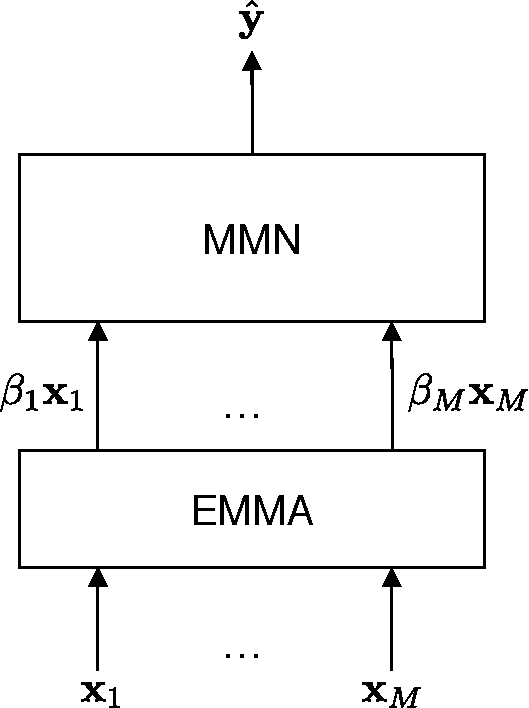
\includegraphics[scale=0.5]{figures/mlp-with-emma}
\caption[High-level view of a Multi-Modal Network with EMMA]{High-level view of a Multi-Modal Network with the EMMA module.}	
\label{fig:mnn-with-emma}
\end{figure}

%----------------------------------------------------------------------------------------
%	SECTION 
%----------------------------------------------------------------------------------------

\section{From Potential to Modal energies (step 2)}\label{sec:step2}
The self-energy is defined as an affine function of the potential energy,
\begin{equation}
e_i = w_i\Psi_i + b_i \qquad \text{with} \qquad w_i \in [1, +\infty],\, b_i \in \mathbb{R}^+,
\label{eq:self-energy}
\end{equation}
where the parameters $w_i$ and $b_i$ are trained via a loss function on the predictions. Therefore, the model is able to capture both the relevance and failure via the self-energy. The second advantage of this transformation is that it helps the module to handle potentials on different numerical scales. Indeed, Equation (\ref{eq:potential-prop}) only guarantees being proportional to the NLL, thus potentials of different modes may not be on comparable scales. The reason the parameters are constrained to be positive will be justified below. Additionally, it will be shown below that self-energies are guaranteed to be positive at the end of this section.

After computing the self-energies, the shared energies can be determined. The expression $e_{ij}$ denotes the shared energy of mode $j$ on $i$ and is constructed from the self-energies as follows
\begin{equation}
e_{ij} = w_{ij}e_i^{\gamma_{ij}}e_j^{1-\gamma_{ij}} \qquad \text{with} \qquad w_{ij} \in [-1,+1],\,\, \gamma_{ij} \in [0,1]
\label{eq:shared-energy}
\end{equation}
where the parameter $\gamma_{ij}$ learns the degree of coupling in the spectrum from strongly coupled ($\gamma_{ij}=0$) to independent ($\gamma_{ij} = 1$). Indeed, if the model learns a value of $\gamma_{ij}$ close to zero, mode $j$ will influence mode $i$ much more than for a $\gamma_{ij}$ close to unity. Equally important is the direction of coupling between mode $i$ and $j$, determined by the weights $w_{ij}$ and $w_{ji}$. We verify that an increase/decrease of the self-energy $e_j$ leads to an increase/decrease of the modal energy $E_i$ for a positive weight $w_{ij}$, and a decrease/increase of $E_i$ for a negative weight $w_{ij}$. This is valid since self-energies are guaranteed to be positive (see next paragraph). The direction of coupling is useful to distinguish modes with redundant or conflicting information from those with complementary information. Notice that the degree and direction of coupling are asymmetric ($\gamma_{ij} \neq \gamma_{ji},\, w_{ij} \neq w_{ji}$). This asymmetry is justified by the following example: take a multi-modal problem with three modes A, B and C. We want the model to learn that if mode A is failing, it is optimal that mode B "takes over". And if mode B is failing, it is optimal for C to "take over". This example can only be modelled with asymmetry. In conclusion, the model has the ability, through the use of shared energies, to discover the different interdependencies between the modes.

A consequence of the design of Equation (\ref{eq:shared-energy}) is that the evaluation of the gradient during the backpropagation step now involves taking the logarithm of $e_i$\footnote{See Appendix \ref{sec:log-gradient}}, which is undefined for negative values. As the weights in Equation (\ref{eq:self-energy}) are positive, we only have to make sure the values of the potential energy are positive. The latter is done by lowering the potential $\Psi_i$ to Euler's number $\mathrm{e}$ as
\begin{equation}
\Psi_i \leftarrow \max(\mathrm{e}, \Psi_i - \Psi_i^{(\text{min})} + \mathrm{e})
\label{eq:correction}
\end{equation}
where $\Psi_i^{(\text{min})}$ denotes the lowest value of $\Psi_i$ in the training set. This correction avoids undefined values ($\Psi_i \geq 0$), exploding gradient\footnote{Exploding gradients are very large gradients, which in turn results in large updates of the network weights, resulting in an unstable network. A good overview on this subject can be found in \citep{exploding}} ($\Psi_i \geq \mathrm{e}$) and guarantees self-energies to be positive. The reason a max-operator is used is because lower energy values than $\Psi_i^{(\text{min})}$  can occur during inference. Clearly, this correction step (\ref{eq:correction}) must be performed prior to the computation of self-energies (\ref{eq:self-energy}).

%----------------------------------------------------------------------------------------
%	SECTION 
%----------------------------------------------------------------------------------------

\section{From Modal energies to Importance scores (step 3)}\label{sec:step3}
The importance scores are computed from the modal energies via the Boltzmann distribution:
\begin{equation}
\alpha_i = \frac{1}{Z}e^{-\rho E_i} \quad \text{with the partition function} \quad Z = \sum_{j=1}^M e^{-\rho E_j} 
\label{eq:gibbs-distrib}
\end{equation}
This guarantees the scores are normalized and sum up to one. A mode $i$ will be said to be important if its score is close to one (low modal energy $E_i$). The hyperparameter $\rho$ represents the coldness, the inverse of the temperature. It controls the entropy of the importance scores distribution. At high temperature ($\rho \rightarrow 0$) the distribution becomes more uniform, and at low temperature ($\rho \rightarrow +\infty$) the importance scores corresponding to the lowest energy tends to 1, while the others approach 0. As can be observed in Figure \,\ref{fig:gibbs}, the coldness has a significant influence on the overall behaviour of the attention module. Hence, careful tuning of $\rho$ is required.

\begin{figure}[!h]
\centering
\begin{subfigure}{.5\textwidth}
  \centering
  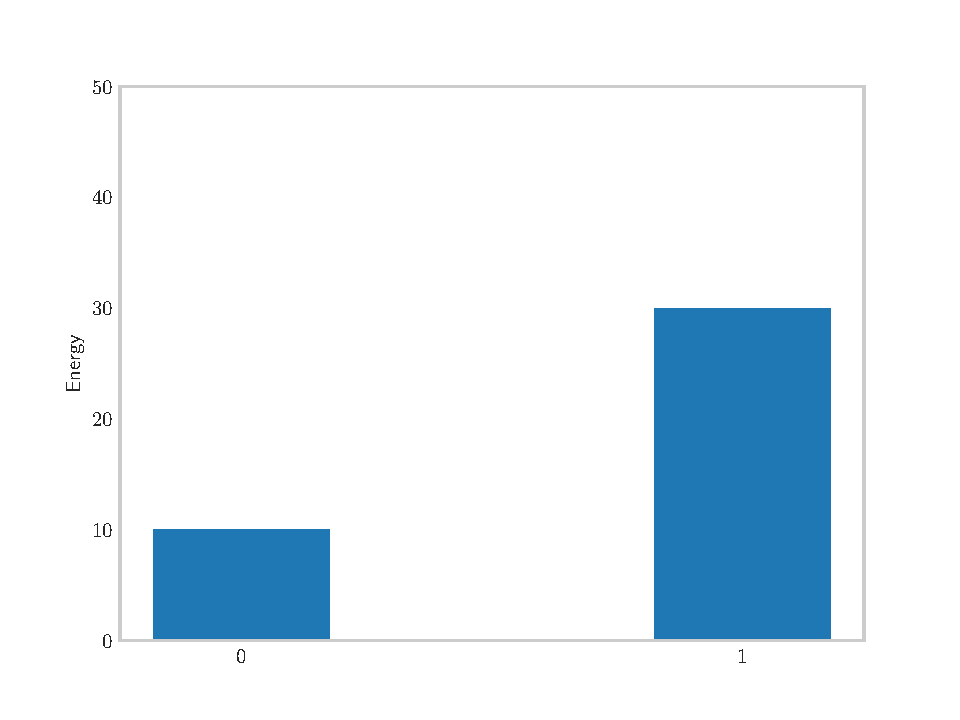
\includegraphics[width=.95\linewidth]{figures/input-gibbs}
  \caption{Energies}
\end{subfigure}%
\begin{subfigure}{.5\textwidth}
  \centering
  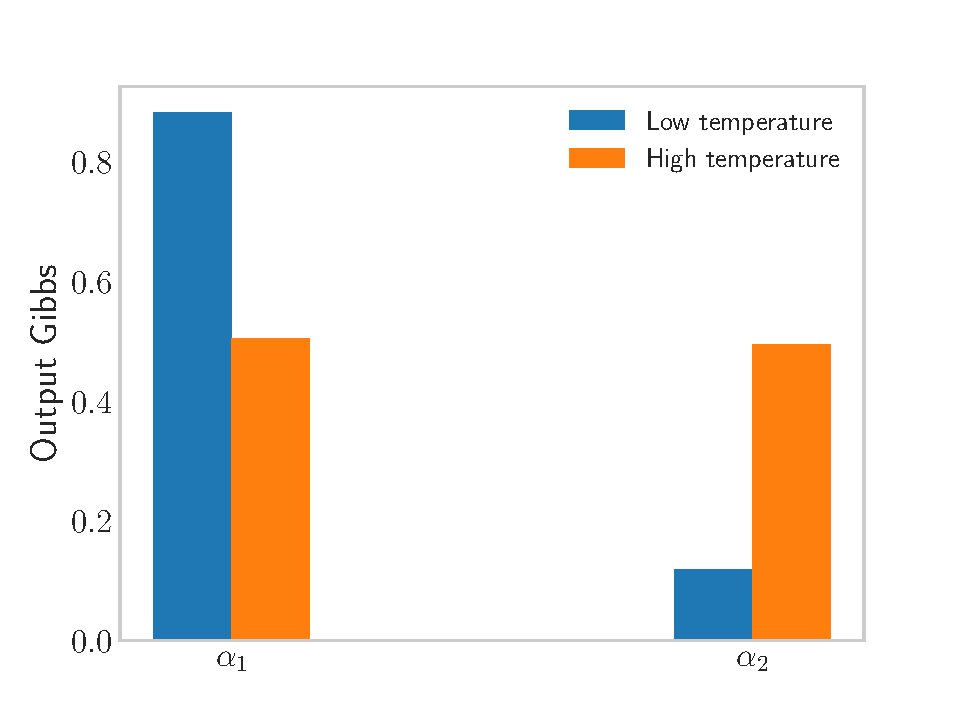
\includegraphics[width=.95\linewidth]{figures/result-gibbs}
  \caption{Importance scores}
\end{subfigure}
\caption[Input-output of Boltzmann distribution for two different temperatures]{Input-output of Boltzmann distribution for two different temperatures, low temperature ($\rho = 0.1$) and high temperature ($\rho = 0.001$)}
\label{fig:gibbs}
\end{figure}


%----------------------------------------------------------------------------------------
%	SECTION 
%----------------------------------------------------------------------------------------

\section{From Importance to Attention scores (step 4)}\label{sec:capacity}
The attention scores are given by
\begin{equation}
\beta_i = \max[0, \tanh(g_a\alpha_i - b_a)] \quad \text{with} \quad g_a > 0,\,\,b_a\in [0,1]
\end{equation}
The hyperbolic tangent adds non-linearity while the gain $g_a$ and bias $b_a$ enable the model to control the threshold and capacity (see Figure \ref{fig:attention-function}). Those two concepts are detailed below.
\begin{figure}[!h]
\centering
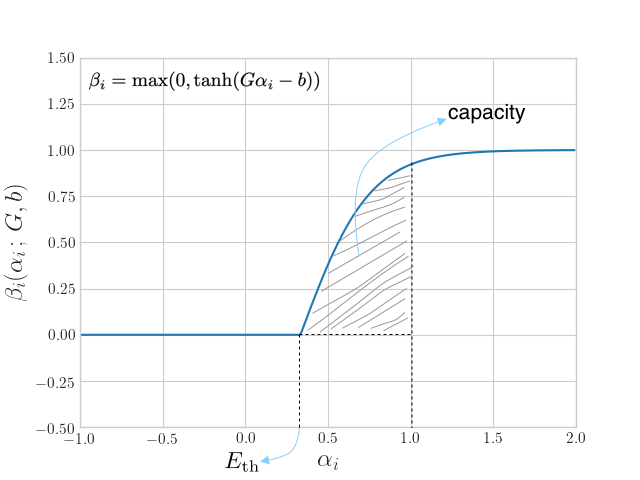
\includegraphics[scale=0.5]{figures/tanh-annotated}
\caption[Attention function]{Attention function (the max-operator generalizes the attention function to cases where $\alpha \in \mathbb{R}$)}
\label{fig:attention-function}
\end{figure}

\subsection*{Energy threshold}
The module will let the information of mode $i$ pass by, only if $g_a\alpha_i - b_a > 0$
\begin{equation}
\begin{split}
&\Leftrightarrow\log(\alpha_i) > \log(b_a/g_a)\\
&\Leftrightarrow E_i \leq \frac{\log(g_a/b_a) - \log(Z)}{\rho} = E_{\text{threshold}}
\end{split}
\end{equation}
where $E_{\text{threshold}}$ represents the maximum energy level for mode $i$ to be taken into account (see Figure \ref{fig:attention-function}). We deduce that the learned gain and bias control this threshold. Notably, the threshold is varying on a per-sample basis due to the partition function $Z$. For example, an increase of the overall perturbation level on the entire input results in a reduction of the partition function, leading to a higher threshold $E_{\text{threshold}}$. It can thus be deduced that EMMA becomes less selective if the overall quality of the sample decreases. 

\subsection*{Capacity}
A more common way to write the attention function would be $\tanh(\mathbf{W}\bm{\alpha}+\mathbf{b})$, whereas we have $\tanh(g_a I\bm{\alpha}-b_a\mathbf{1})$, where $I$ is the identity matrix. We argue the latter better mimics human's attention, permitting us to introduce the concept of capacity, which in psychology is viewed as the amount of resource that can be allocated \citep{attention-is-effort}. If we look at Figure \ref{fig:attention-function}, this can be translated as,
\begin{equation}
\text{capacity} \triangleq \int_0^1 \tanh(g_a\alpha - b_a)d\alpha 
\end{equation}
Define the auxiliary variable $u = g_a\alpha - b_a$. Now using
\begin{equation}
\frac{du}{d\alpha} = g_a \Leftrightarrow d\alpha = \frac{1}{g_a}du
\end{equation}
we can write 
\begin{equation}
\begin{split}
\text{capacity} &= \frac{1}{g_a} \int_{-b_a}^{g_a-b_a} \tanh(u)du  \\
&= \frac{1}{g_a}\log[\cosh(u)]\bigg\rvert_{-b_a}^{g_a-b_a} + \cancel{\text{constant}} \\
&= \frac{1}{g_a}\log\bigg[\frac{\cosh(g_a - b_a)}{\cosh(-b_a)}\bigg]
\end{split}
\label{eq:capacity}
\end{equation}
When the capacity is too low, no sufficient amount of information is passed to the MMN, leading to wrong predictions. Similarly, if the capacity is too high, the perturbations of the failing modes will pass and cause a decrease in performances. It is expected that the model learns the optimal trade-off. However, if we want the attention module to be robust against failing situations it was not trained on, we suggest minimizing capacity would result in appealing properties for the system as a whole. The reasons for minimizing the capacity are two-fold: it forces the module to mask out more information, which may be sub-optimal on the training set but useful to generalize against more intensive failing modes. The second reason is to avoid the extreme case where the module leaves all the inputs unchanged (maximal capacity) and instead it is the MMN who learns to suppress perturbations. The ideal method for controlling the capacity, would be to add the derived expression (\ref{eq:capacity}) as a regularizer to the loss function, but this could potentially lead to instabilities\footnote{The gradient of Equation (\ref{eq:capacity}) can become very large for certain values of its weights $g_a$ and $b_a$.} during training. A less precise but more stable way is to introduce the expression $g_a-b_a$ instead in the loss function. We verify that minimizing this expression will minimize the gain while maximizing the bias, i.e. lead to a decrease of the capacity. Nevertheless, Equation (\ref{eq:capacity}) can still be used to compute the learned capacity of the module. Notice that the concept of capacity can also be applied to $\tanh(W\bm{\alpha}+\mathbf{b})$, but in this case each mode would have his own capacity, making the importance scores less meaningful.


%----------------------------------------------------------------------------------------
%	SECTION 
%----------------------------------------------------------------------------------------

\section{Training \& Regularization}\label{sec:regul}
The training of the attention module and the prediction model is performed in two stages (see Figure \ref{fig:training}). First, each mode is assigned a separate autoencoder, which is trained on the mode to learn the potential energy function. Once trained, the weights of the autoencoders are frozen. In the second phase, EMMA is inserted in front of the MMN and is trained end-to-end on both normal and corrupted data. By corrupted data, we mean samples on which a corruption process is applied in order to simulate one or more failing modes. Notably, the computational overload induced by the training of EMMA in the second stage is often negligible with respect to the MMN, provided that the number of parameters of EMMA\footnote{The number of parameters of EMMA scales up quadratically with the number of modes.} is in most cases far less than the number of parameters of the MMN. 

Additionally, two regularizers are introduced in the loss function, written as
\begin{equation}
\tilde{\mathcal{L}} = \mathcal{L}(y,\hat{y}) + \lambda_c(g_a-b_a) - \lambda_e \Omega \quad \text{with} \quad \Omega = \sum_{k=1}^M \xi_k \log(\alpha_k) \quad \text{and} \quad \xi_k = \begin{cases}
      \xi_- = -1 & \text{if}\ \mathbf{x}_k\, \text{is corrupted} \\
      \xi_+ = +1 & \text{otherwise}
    \end{cases}
\label{eq:regularization}
\end{equation}
with $\lambda_c$ and $\lambda_e$ being positive real numbers used to set the relative importance of each regularizer, and the $\xi_k$ vector being manually encoded. The first regularizer minimizes the capacity, where a higher $\lambda_c$ pushes the module to let less information pass through in general (i.e., to be more "cautious"). The second regularizer ($\lambda_e \Omega$), which we call the energy regularizer, controls the trade-off between on the one hand the coupling and on the other hand the failure intensity. In use-cases with complex asymmetric interactions between the modes, the shared energies could potentially cause large discrepancies between modal energies $E_i$ and their original potential energies $\Psi_i$. A major drawback of having such discrepancies is that this leads to a reduction of the influence of the failure intensity in the computation of the attention scores. This may result in poor generalization to samples with more intensive failing modes. We show that these discrepancies can be reduced to a certain degree by the use of the energy regularizer. Indeed, as an effect of this regularizer, modal energies with low/high potential energies (uncorrupted/corrupted modes) will be decreased/increased. Although the energy regularizer is relatively straightforward, we will demonstrate below that some care needs to be taken regarding the corruption process.

\subsection*{Energy regularization}
Let $\bm{\theta} = \{\bm{\theta}_1\ldots\bm{\theta}_M\}$ be the set of all the parameters of the second step\footnote{See Section \ref{sec:step2}} of the attention module, where $\bm{\theta}_i = \{[\gamma_{ij}, w_{ij}]_{j=1}^M, w_i, b_i\}$ are the parameters composing the modal energy $E_i$. The effect of the energy regularizer in the SGD algorithm is isolated and written
\begin{equation}
\bm{\theta} \leftarrow \bm{\theta} + \epsilon\lambda_e\nabla_{\bm{\theta}}\Omega
\label{eq:update}
\end{equation}
Remember that the objective is to update the parameters such that for low/high potential energies $\Psi_i$ the modal energies $E_i$ are decreased/increased. To verify this let us compute\footnote{The batch is assumed to only contain one sample for the sake of simplicity. However, the demonstration can be generalized to any batch size.} $\nabla_{\bm{\theta}}\Omega$,
\begin{equation}
\nabla_{\bm{\theta}} \Omega =\sum_{k=1}^M \xi_k \nabla_{\bm{\theta}} \log(\alpha_k) 
\label{eq:dev}
\end{equation}
The gradient of the logarithm can be developed as
\begingroup
\allowdisplaybreaks
\begin{align*}
\nabla_{\bm{\theta}}  \log(\alpha_k) &= \nabla_{\bm{\theta}} \log \bigg[ \frac{e^{-\rho E_k}}{Z} \bigg] \\*
&=  \nabla_{\bm{\theta}}(-\rho E_k) -  \nabla_{\bm{\theta}} \log \sum_{l=1}^M e^{-\rho E_l} \\*
&=  -\rho \nabla_{\bm{\theta}}E_k - \frac{\sum_{l=1}^M \nabla_{\bm{\theta}} e^{-\rho E_l}}{\sum_{l=1}^M e^{-\rho E_l}} \\
&= -\rho \nabla_{\bm{\theta}}E_k + \rho \frac{\sum_{l=1}^M e^{-\rho E_l} \nabla_{\bm{\theta}}E_l}{\sum_{l=1}^M e^{-\rho E_l}} \\
&= \rho \Bigg[ -\big(1 - \frac{e^{-\rho E_k}}{Z}\big)\nabla_{\bm{\theta}}E_k + \sum_{l \neq k}^M \frac{e^{-\rho E_l}}{Z} \nabla_{\bm{\theta}}E_l \Bigg] \\
&= \rho \Bigg[ -\big(1 - \alpha_k\big)\nabla_{\bm{\theta}}E_k + \sum_{l \neq k}^M \alpha_l \nabla_{\bm{\theta}}E_l \Bigg] \\
\label{eq:grad-log}
\end{align*}
\endgroup
%\begin{equation}
%\begin{split}  
%\end{split}
%\end{equation}

We go further by expressing the equation above with respect to the subset of parameters $\bm{\theta}_i$:
\begin{equation}
\nabla_{\bm{\theta}_i}  \log(\alpha_k) = \begin{cases}
      -\rho(1-\alpha_i)\nabla_{\bm{\theta}_i}E_i, & \text{if}\, i = k \\
       \rho\alpha_i\nabla_{\bm{\theta}_i}E_i, & \text{if}\, i \neq k
    \end{cases}
\label{eq:log-split}
\end{equation}

The gradient of the regularizer can now be computed by plugging Equation (\ref{eq:log-split}) into the summation (\ref{eq:dev}). Let $M'$ be the number of uncorrupted modes. We obtain for an uncorrupted mode $i$,
\begin{equation}
\nabla_{\bm{\theta}_i}\Omega = \xi_+\big[ -\rho(1-\alpha_i)\nabla_{\bm{\theta}_i}E_i \big] + \big[(M'-1)\xi_+ + (M-M')\xi_-\big]\alpha_i\rho\nabla_{\bm{\theta}_i}E_i
\label{eq:normal-exp}
\end{equation}
and for a corrupted mode $i$,
\begin{equation}
\nabla_{\bm{\theta}_i}\Omega =\xi_-\big[ -\rho(1-\alpha_i)\nabla_{\bm{\theta}_i}E_i \big] + \big[M'\xi_+ + (M-M'-1)\xi_-\big]\alpha_i\rho\nabla_{\bm{\theta}_i}E_i
\label{eq:abnormal-exp}
\end{equation}
We can summarize Equations (\ref{eq:normal-exp}) and (\ref{eq:abnormal-exp}) as
\begin{equation}
\boxed{\nabla_{\bm{\theta}_i}\Omega = -\big[(M-2M')\alpha_i + \xi_i\big]\rho\nabla_{\bm{\theta}_i}E_i}
\end{equation}


Adding the constraint that $M' = \lfloor \frac{M+1}{2} \rfloor$, two cases can be distinguished. If the total number of modes $M$ is even, then we have
\begin{equation}
\bm{\theta}_i \leftarrow \bm{\theta}_i - \epsilon\lambda_e\rho\xi_i\nabla_{\bm{\theta}_i}E_i \quad \text{with} \quad \lambda_e \in \mathbb{R}^+
\label{eq:update-param}
\end{equation}
The value of the modal energy function for the updated parameters can be developed with a first-order Taylor series approximation around the prior-to-update parameter set $\bm{\theta}_i^{(0)}$, with a fixed input $\mathbf{x}_i$:
\begin{equation}
E_i\big(\mathbf{x}_i;\bm{\theta}_i\big) \approx E_i\big(\mathbf{x}_i;\bm{\theta}_i^{(0)}\big) + \big(\bm{\theta}_i - \bm{\theta}_i^{(0)}\big)^T\nabla_{\bm{\theta}_i}E_i
\end{equation}
Substituting the updated parameters (\ref{eq:update-param}) into our approximation, we obtain
\begin{equation}
E_i\big(\mathbf{x}_i;\bm{\theta}_i^{(0)} - \epsilon\lambda_e\rho\xi_i\nabla_{\bm{\theta}_i}E_i\big) \approx E_i\big(\mathbf{x}_i;\bm{\theta}_i^{(0)}\big) - \epsilon\lambda_e\rho\xi_i\big(\nabla_{\bm{\theta}_i}E_i\big)^T\nabla_{\bm{\theta}_i}E_i
\end{equation}
where the left-hand side corresponds to the energy value with the updated parameters, and the first term of the right-hand side corresponds to the energy value before the parameter update. Using the fact that $\xi_i$ is negative (resp.\ positive) for a corrupted (resp.\ uncorrupted mode), it can be concluded from the equation above that the regularizer will update the parameters such that the values of the modal energy function $E_i$ increases (resp.\ decreases) for a same sample of the corrupted (resp.\ uncorrupted mode) $i$.

In analogy, if M is odd we have
\begin{equation}
\bm{\theta}_i \leftarrow \begin{cases}
       \bm{\theta}_i - \epsilon\lambda_e\rho(1-\alpha_i)\nabla_{\bm{\theta}_i}E_i, & \text{if $i$ is uncorrupted} \\
       \bm{\theta}_i + \epsilon\lambda_e\rho(1+\alpha_i)\nabla_{\bm{\theta}_i}E_i & \text{otherwise}
    \end{cases}
\end{equation}
The principle is the same as in the even case with an additional effect: the correction will be proportional to the error. To put it in another way, high energies that must be low and low energies that have to be high will have stronger gradients than their counterparts. This is similar to the positive and negative phase in the optimization of Restricted Boltzmann Machines.

To conclude, let us notice that some undesired effects can appear if we do not add the constraint $M' = \lfloor \frac{M+1}{2} \rfloor$. As an illustration, take $M' = \lfloor \frac{M+1}{2} \rfloor + 1$, Equation (\ref{eq:update}) becomes
\begin{equation}
\bm{\theta}_i \leftarrow \bm{\theta}_i - \epsilon\lambda_e\rho(\alpha_i + \xi_i)\nabla_{\bm{\theta}_i}E_i
\end{equation}
which is unstable for uncorrupted modes leading to a collapse where all energies tend to decrease.

%----------------------------------------------------------------------------------------
%	SECTION 
%----------------------------------------------------------------------------------------

\section{Advantages}
The key advantages of using EMMA are:
\begin{itemize}
\item The generic design of EMMA permits it to be easily added to any type of architecture of a multi-modal model, without modifying nor EMMA nor the MMN.
\item The burden on the MMN is reduced, it only has to learn to make good predictions from the received information. The MMN does not need anymore to learn to distinguish failing modes.
\item Our attention module improves the interpretability of the overall model in two ways. First, it can be verified on a per-sample basis which modes are failing and important. Secondly, the \textit{total energy}, $\sum_i E_i$, provides us with an approximate measure of the uncertainty on the predictions (see Section \ref{sec:total-energy}). A useful concrete application, would be to use these interpretable clues to trigger specific hardware/software recovery systems (e.g., luminosity calibration of camera in self-driving cars).
\end{itemize}

%\newpage
\null
\vfill
\begin{center}
\begin{figure}[!h]
\centering
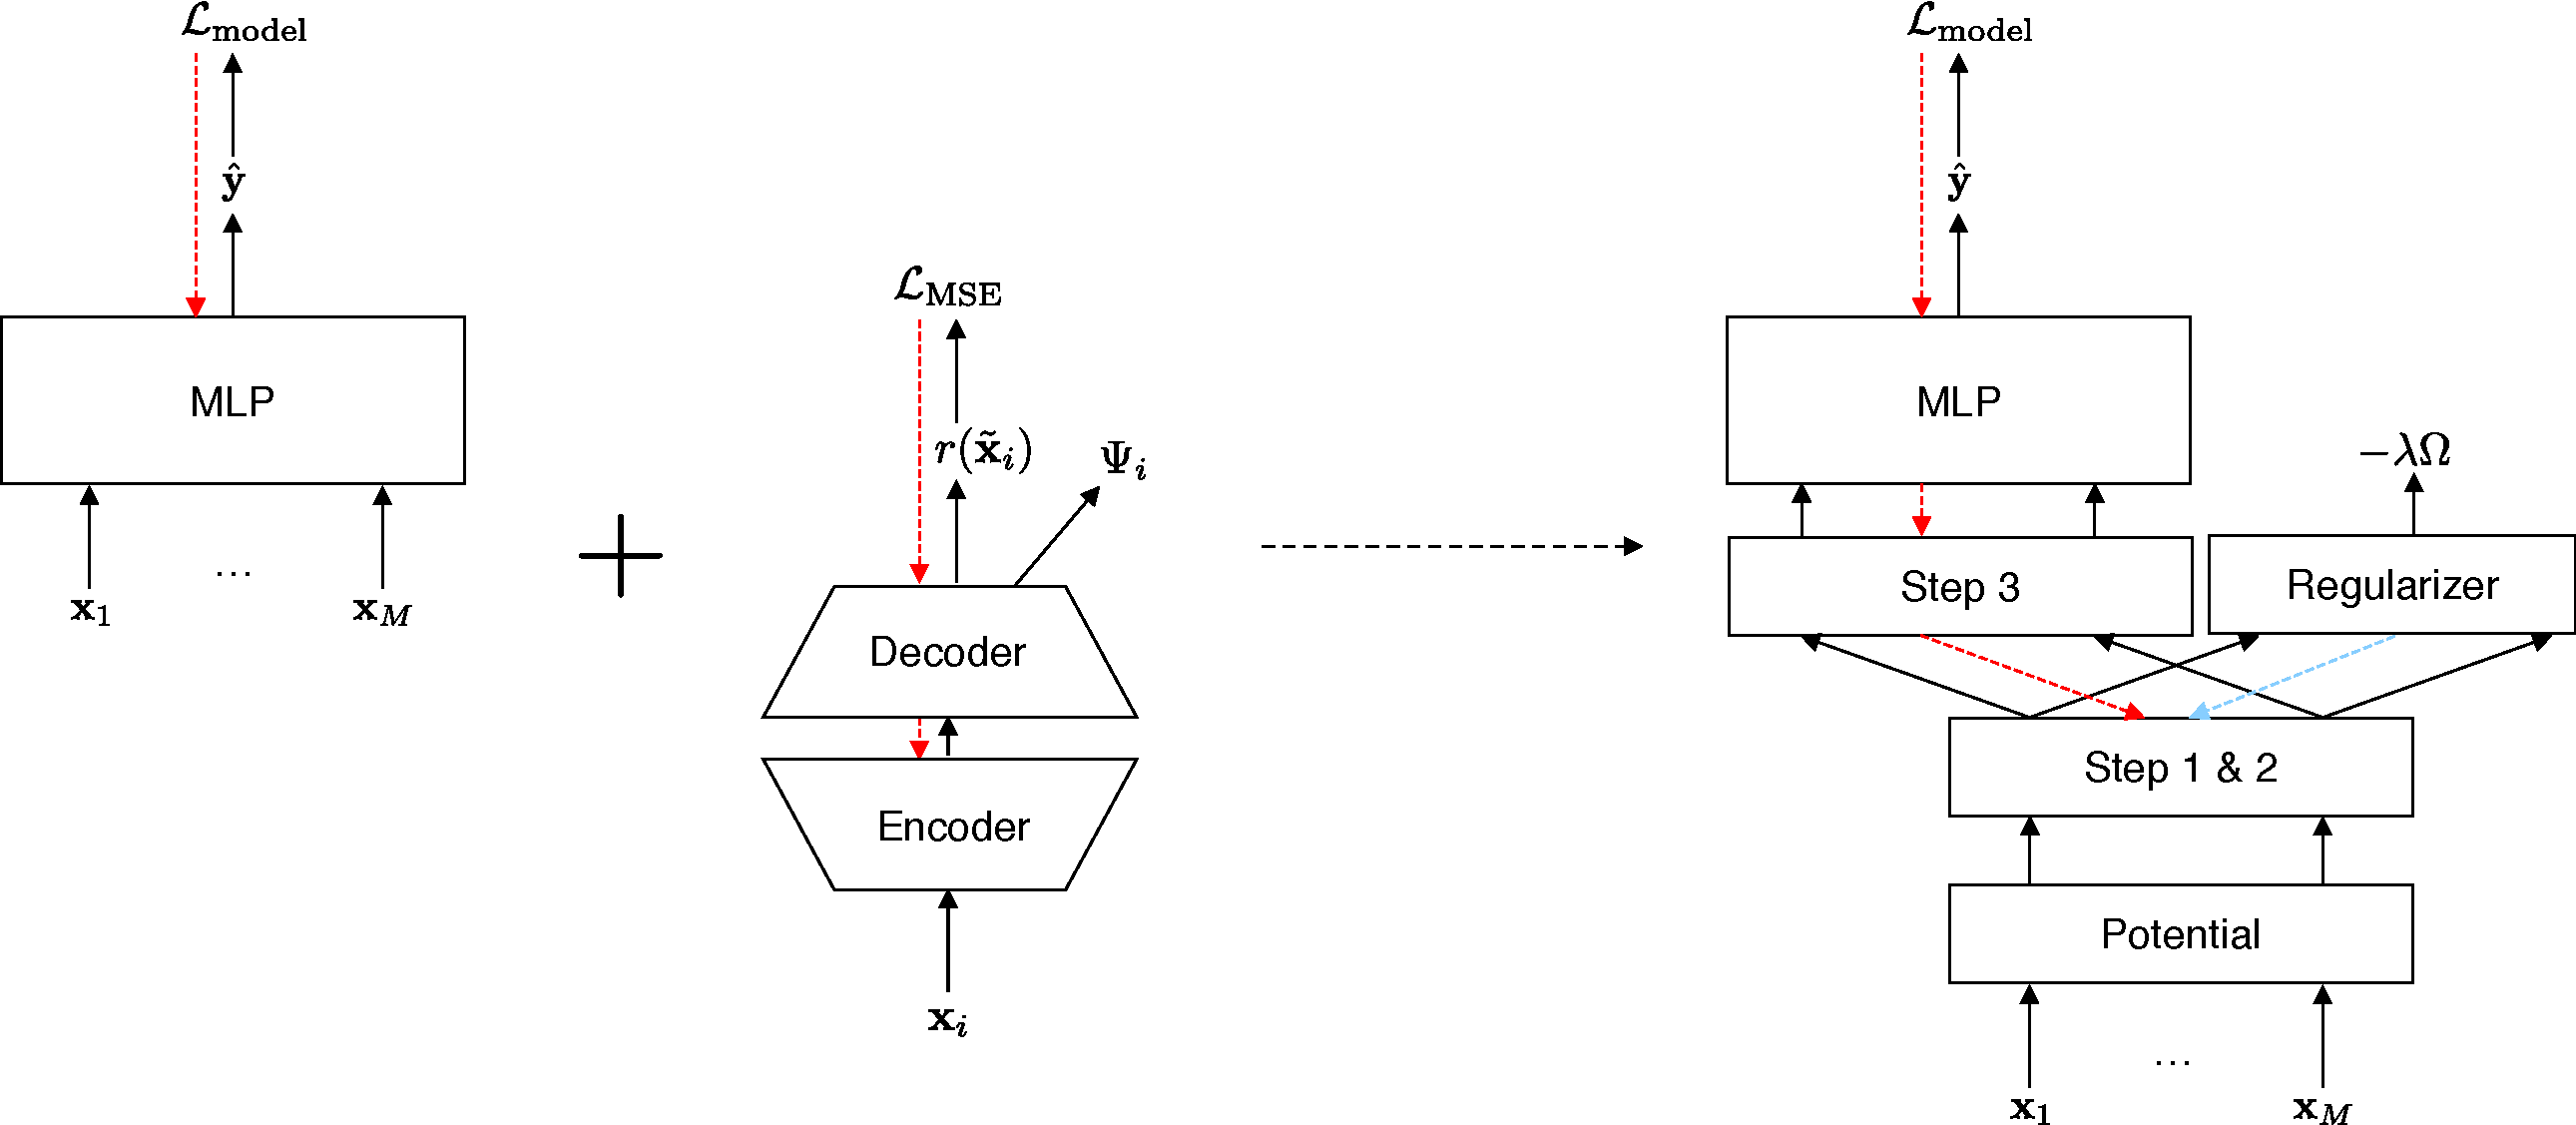
\includegraphics[scale=0.5]{figures/summary-training}
\caption{Summary of end-to-end training.}	
\label{fig:training}
\end{figure}
\end{center}
\vfill
\clearpage 
\chapter{Experiments \& Results} 
\label{chapter-experiments} 

Both are experiments on dataset described in previous chapter. Experiment II will be about energy estimation. Experiment III evaluates and analyzes the robustness of the model with and without EMMA.


%----------------------------------------------------------------------------------------
%	SECTION 
%----------------------------------------------------------------------------------------

\section{Pulsar detection}
The models will be trained to detect pulsar stars. In (very) short, pulsar stars are neutron stars emitting radio waves on a periodic time-frame. A summary of the seminal work of \citep{lyon} can be found in Appendix \ref{chapter-dataset}. The thesis can be accessed \href{http://www.scienceguyrob.com/wp-content/uploads/2016/12/WhyArePulsarsHardToFind_Lyon_2016.pdf}{here}\footnote{\url{http://www.scienceguyrob.com/wp-content/uploads/2016/12/WhyArePulsarsHardToFind_Lyon_2016.pdf}} and the dataset \href{https://archive.ics.uci.edu/ml/datasets/HTRU2}{here}\footnote{\url{https://archive.ics.uci.edu/ml/datasets/HTRU2}}.

Short description of two modes (ip and dm) and internal features (mean...).  Explain why detection is difficult. Classification signal/background. Skewed dataset, give numbers.

%----------------------------------------------------------------------------------------
%	SECTION 
%----------------------------------------------------------------------------------------

\section{Corruption}
\begin{itemize}
\item standardize, why? split sets and apply one from train \href{https://stats.stackexchange.com/questions/327294/data-standardization-for-training-and-testing-sets-for-different-scenarios}{error standardize}
\item SNR (see good explanation in pulsar thesis). If greater than 1, signal non-distinguishable. White noise. Explain it is not the same than AE corruption. $ 10\log(\frac{1}{\sigma^2})$
\item on signal and background because we corrupt the whole mode and not the class
\end{itemize}


%----------------------------------------------------------------------------------------
%	SECTION 
%----------------------------------------------------------------------------------------

\section{Experiment II}

\begin{itemize}
\item train-test split
\item AE trained on train-set and then test on test-set
\item matrix with number of signals, ... (eda)
\end{itemize}

Setup: max epochs = 30, batch size = 64, noise DAE = 0.01, d input = 4, n hidden = 12, adam 0.001, sigmoid

\begin{figure}[!h]
\centering
\begin{subfigure}{.5\textwidth}
  \centering
  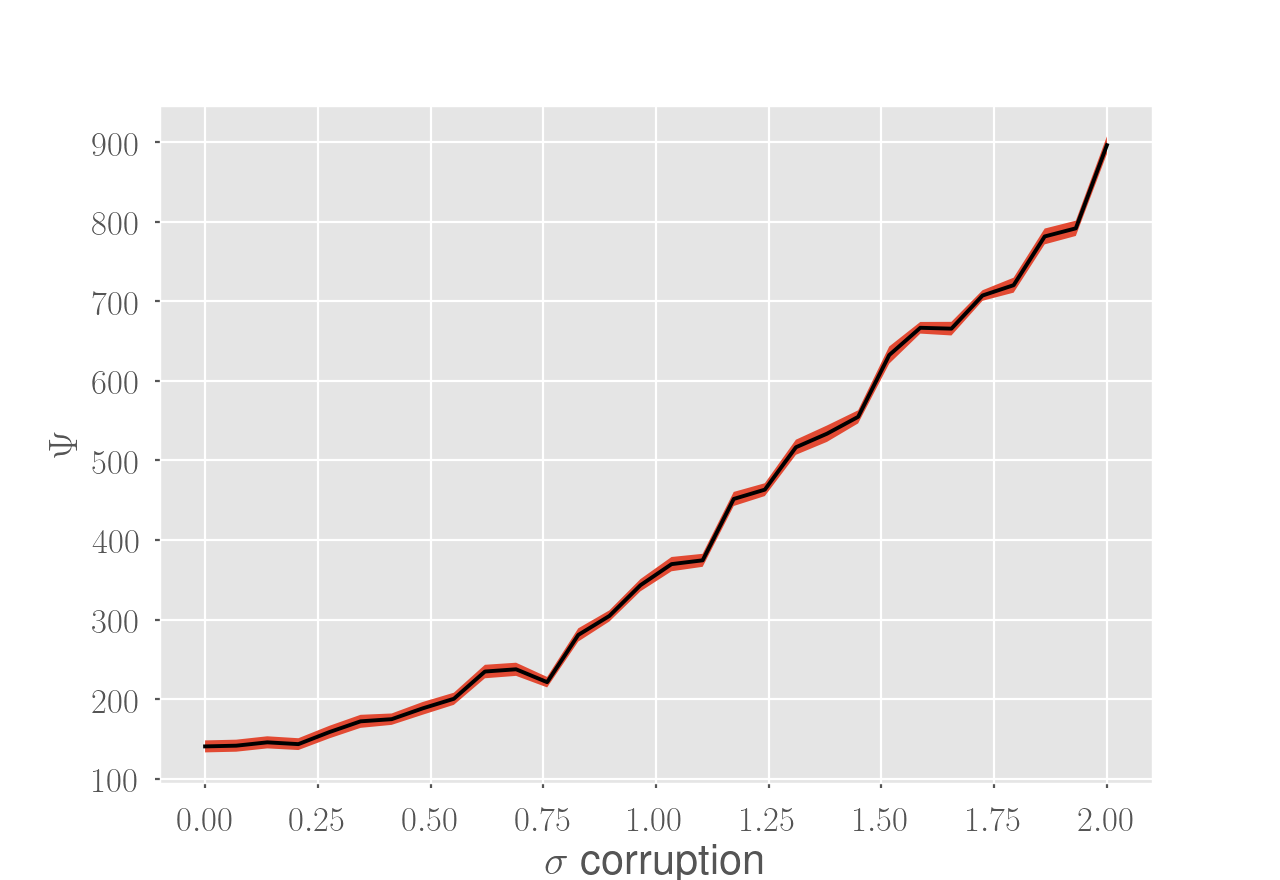
\includegraphics[width=\linewidth]{figures/noisy-signal-ip}
\end{subfigure}%
\begin{subfigure}{.5\textwidth}
  \centering
  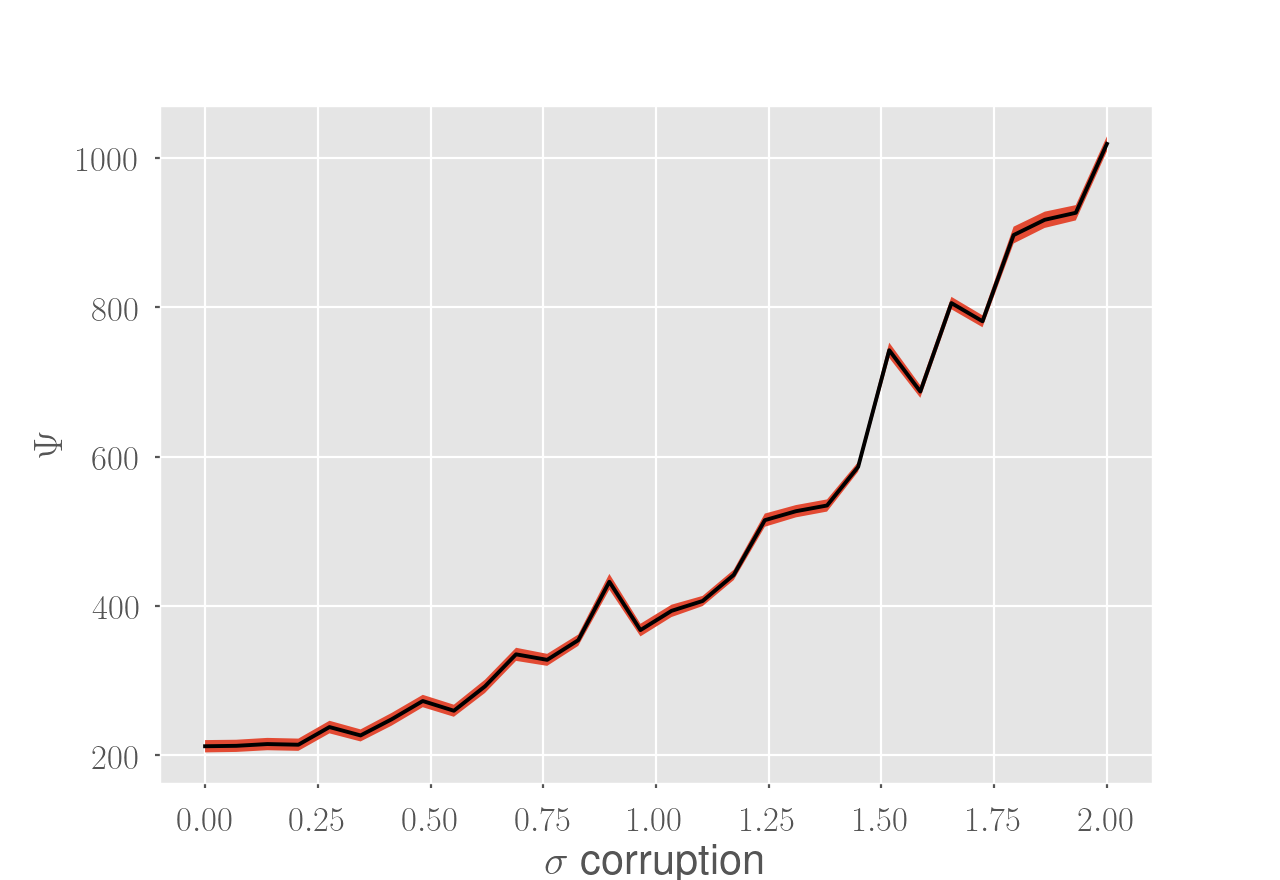
\includegraphics[width=\linewidth]{figures/noisy-signal-dm-snr}
\end{subfigure}
\end{figure}


%----------------------------------------------------------------------------------------
%	SECTION 
%----------------------------------------------------------------------------------------

\section{Experiment III}

\begin{itemize}
\item BCE \& F1 (not AUC -- explain why). \href{https://stats.stackexchange.com/questions/210700/how-to-choose-between-roc-auc-and-f1-score}{F1vsAUC1}. \href{https://www.quora.com/What-does-it-mean-to-have-high-AUC-but-low-F1-score}{F1vsAUC2}. \href{https://stackoverflow.com/questions/44172162/f1-score-vs-roc-auc}{F1vsAUC3}. \href{https://www.mikulskibartosz.name/f1-score-explained/}{F1}
\item train-valid-test
\item threshold optimal choice via ROC. all on valid set
\item 3 models: base (train normal, valid normal), without (train noisy, valid noisy), with (train noisy, valid noisy)
\item 50-25-25 noisy mode. give detailed numbers. eda.
\item trained with early stopping + retrain for .. epochs with valid+train. saved model.
\item one subsection per plot: explain details experiment and how results are obtained. then analyze and conclusions.
\end{itemize}

%\begin{landscape}
%\begin{table}
%\centering
%
%\begin{tabular}{@{}lccccccccc@{}}
%\toprule
%Model &  \multicolumn{3}{c}{$F_1$-Scores} & \multicolumn{3}{c}{Precision} & \multicolumn{3}{c}{Recall}  \\
%\cmidrule(lr){2-4}  \cmidrule(lr){5-7}   \cmidrule(lr){8-10} 
%& uncorrupted & noisy-ip & noisy-dm & uncorrupted & noisy-ip & noisy-dm & uncorrupted & noisy-ip & noisy-dm \\
%\midrule
%Without &  \\ %\cline{1-4}
%\hspace*{\fill}Glasses        & 76.78\% & 70.91\% & 74.17\%& 75.95\% & 76.12\% & 76.04\%& 75.95\% & 76.12\% & 76.04\%  \\ %\cline{1-4}
%With& \\ %\cline{1-4}
%Night-BareFace & 80.66\% & 72.11\% & 77.16\%& 75.95\% & 76.12\% & 76.04\%& 75.95\% & 76.12\% & 76.04\%  \\ %\cline{1-4}
%Night-Glasses  & 74.20\% & 81.66\% & 78.56\%& 75.95\% & 76.12\% & 76.04\% & 75.95\% & 76.12\% & 76.04\% \\ \addlinespace %\cline{1-4}
%Overall        & 75.81\% & 75.65\% & 75.73\%& 75.95\% & 76.12\% & 76.04\%& 75.95\% & 76.12\% & 76.04\% \\ 
%\bottomrule
%\end{tabular}
%\caption{Experimental results}
%\label{my-label}
%\end{table}
%\end{landscape}




  
\subsection*{Attention-shift}
\begin{figure}[!h]
\centering
\begin{subfigure}{.5\textwidth}
  \centering
  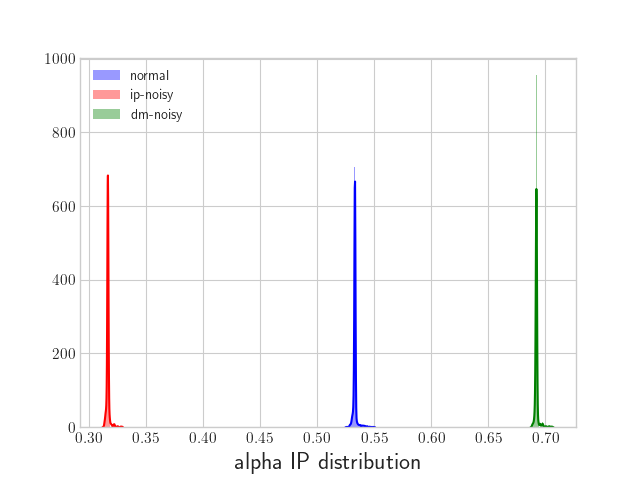
\includegraphics[width=\linewidth]{figures/alpha-distrib-high-cap}
\end{subfigure}%
\begin{subfigure}{.5\textwidth}
  \centering
  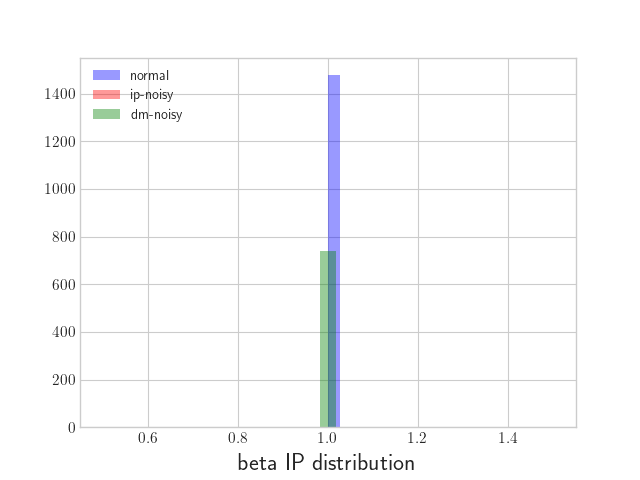
\includegraphics[width=\linewidth]{figures/beta-distrib-high-cap}
\end{subfigure}
\end{figure}

\begin{figure}[!h]
\centering
\begin{subfigure}{.5\textwidth}
  \centering
  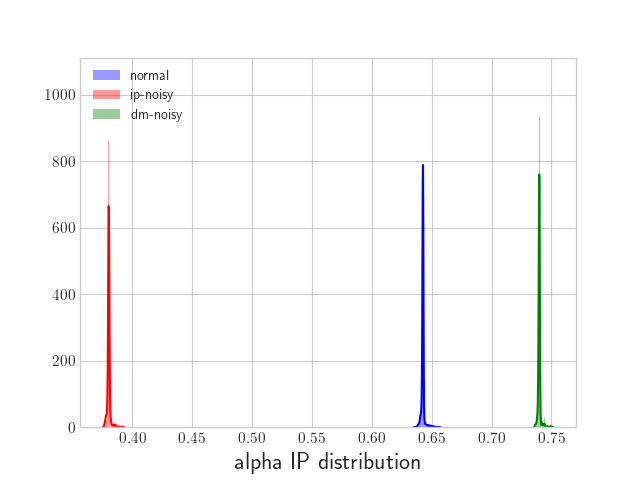
\includegraphics[width=\linewidth]{figures/alpha-distrib-low-cap}
\end{subfigure}%
\begin{subfigure}{.5\textwidth}
  \centering
  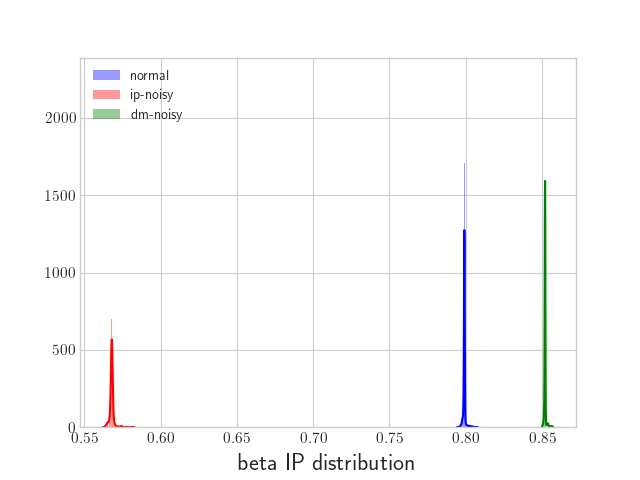
\includegraphics[width=\linewidth]{figures/beta-distrib-low-cap}
\end{subfigure}
\end{figure}


\subsection*{Robustness generalisation}
\begin{figure}[!h]
\centering
\begin{subfigure}{.5\textwidth}
  \centering
  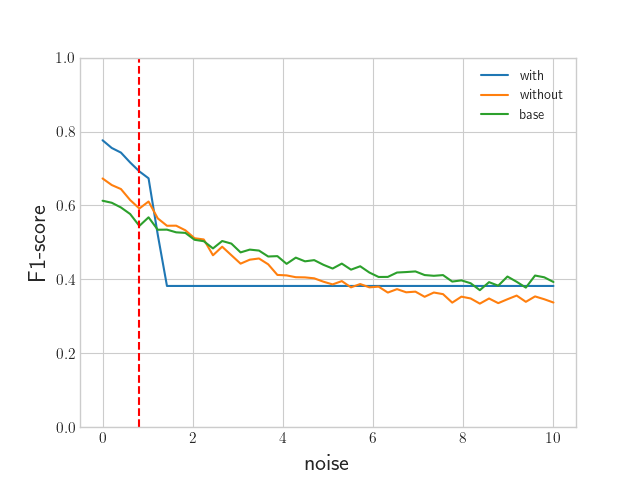
\includegraphics[width=\linewidth]{figures/noise-generalisation-bad-model-0}
\end{subfigure}%
\begin{subfigure}{.5\textwidth}
  \centering
  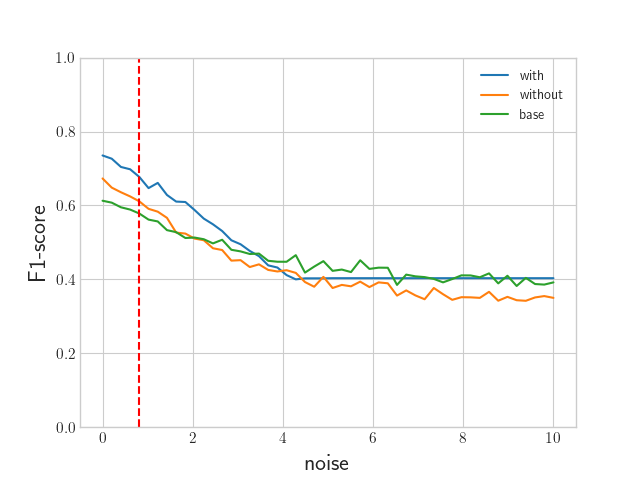
\includegraphics[width=\linewidth]{figures/noise-generalisation-good-model-6}
\end{subfigure}
\end{figure}

\subsection*{Yerkes-Dodson curve}
over-under arousal. do on larger range.
\begin{figure}[!ht]
\centering
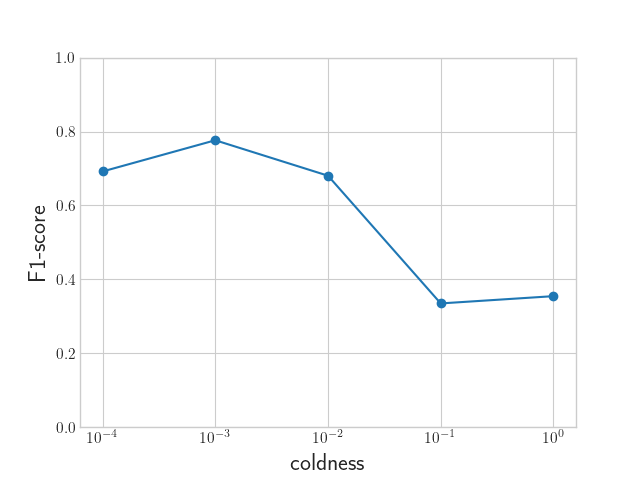
\includegraphics[scale=0.5]{figures/yerkes-dodson}
\end{figure}

\subsection*{Energy generalisation}
\begin{figure}[!ht]
\centering
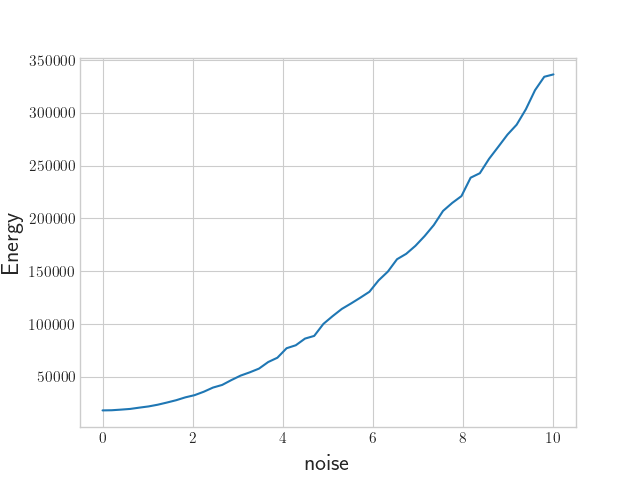
\includegraphics[scale=0.5]{figures/total-energy-model-1}
\end{figure}

 
\chapter{A Unified Model for Multi-Modal Attention} 
\label{chapter-unified} 

The purpose of using EMMA is to help the multi-modal network (MMN) to handle failing modes, and more generally, to figure out the relative emphases to be placed on the different modes depending on their general contributions to the predictions. The literature review\footnote{See Chapter \ref{chapter-literature-review}} discussed self-attention and cross-modal attention mechanisms, used to highlight information inside a specific mode, such as certain regions in an image or a set of frequencies in a sound. The difference between these two mechanisms is that self-attention only relies on information from the mode itself as a context, whereas cross-modal attention uses information from all the available modes. Now that we have EMMA, we claim to have all the ingredients to construct a complete multi-modal network like humans. As a reminder, human's complete multi-modal attention consists of three different components: exogenous, endogenous and cross-modal attention. The endogenous component of attention stems from a conscious, voluntary process, whereby a human elects to focus on a particular object \citep{crossmodal}. In contrast, the exogenous attention is triggered by the sudden onset of an unexpected event, and can thus be viewed as a reaction to an external stimulus \citep{crossmodal}. One way of constructing an endogenous module would be as a block of $M$ self-attentions, where each self-attention is dedicated to one specific mode. On the other hand, the attention module developed in this work can be interpreted as reproducing the exogenous attention used by humans to robustly handle abnormal situations.

\begin{figure}[hbt!]
\centering
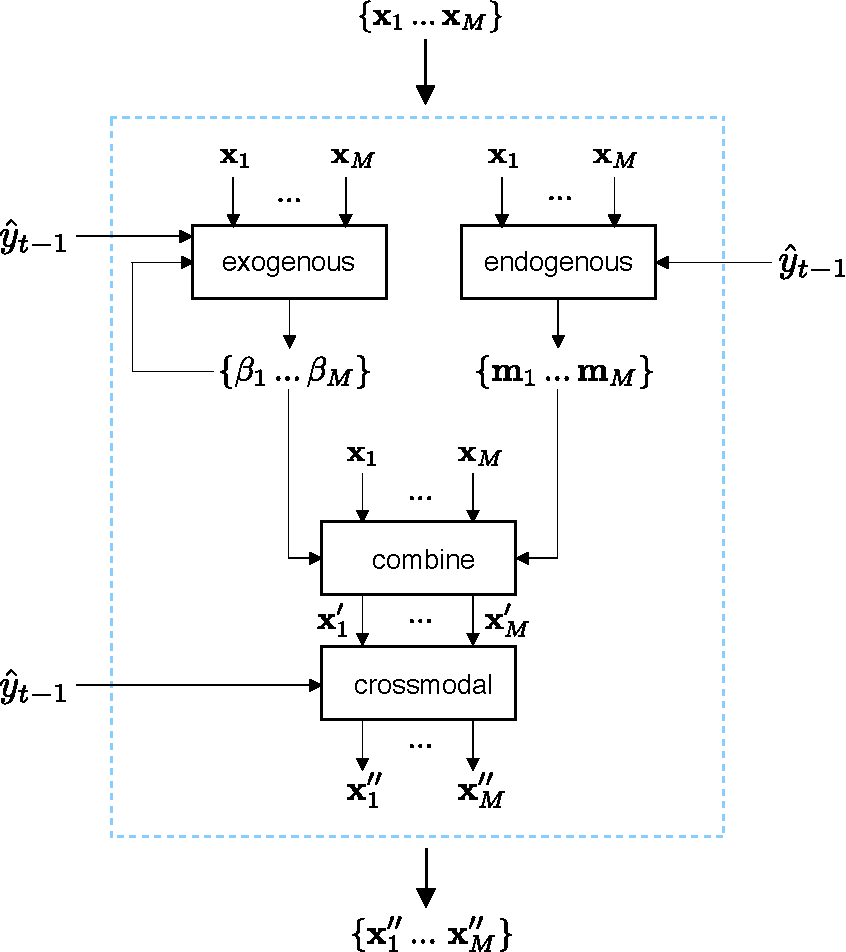
\includegraphics[scale=0.75]{figures/unified}
\caption{A possible architecture for a unified multi-modal attention.}
\label{fig:complete-model}
\end{figure}

With this in mind, we present a unified model (see Figure \ref{fig:complete-model}) combining all the strengths of each type of attention. First, the attention masks $\beta_i$ computed by the exogenous model, and the attention masks $\mathbf{m}_i$ computed by the endogenous module, are combined to obtain the resulting masks $\beta_i\mathbf{m}_i$. These mask will highlight the most important modes, and on an intra-modal level attend to the most relevant regions. The masks $\beta_i\mathbf{m}_i$ are then applied to the input sample, which is passed through the cross-modal module. Finally, the processed input $\{\mathbf{x}''_1\,...\,\mathbf{x}''_M\}$ is forwarded to the MMN. In addition, the complete module can further be refined by inserting feedback loops from the previously predicted output to the separate modules, as it is often done in the literature \citep{afouras, attention-need, bahdanau}. For example, in a self-driving system, the attention module could improve its focus to different regions of the input image depending on the previously detected cars. It is worth mentioning that the proposed architecture is only a generalization of current attention modules such as in \citep{afouras}, supplemented with an exogenous component.


 
\chapter{Conclusion} 
\label{chapter-conclusion} 

Summary of what was seen/done during the master thesis from start to end. Scales up quadratically with number of modes, explain.

%----------------------------------------------------------------------------------------
%	SECTION 
%----------------------------------------------------------------------------------------

\section{Contributions}
Summarize contributions


%----------------------------------------------------------------------------------------
%	SECTION 
%----------------------------------------------------------------------------------------

\section{Research questions}
Each research question + answer


%----------------------------------------------------------------------------------------
%	SECTION 
%----------------------------------------------------------------------------------------

\section{Future work}
\begin{itemize}
\item Annealing + init, end temperature + explain init of next layer \href{http://what-when-how.com/artificial-intelligence/a-comparison-of-cooling-schedules-for-simulated-annealing-artificial-intelligence/}{Linke annealing}. Multiple modes then blows up. Image 100 modes (altough not realistic in real-world problems) then tend to zero. Solution add a common gain? Analyze influence of multiple modes etc..

\item Explore different shared energies design

\item Images/sound sequences. early, late fusion, manifold with respect to unified model? it could be very easy to test on images/sounds (give even during test-time a true outlyingness measure, not specifically the NLL) and at the same time investigate general ways of getting such a measure.

\item Unseen values
\end{itemize}


 

%----------------------------------------------------------------------------------------
%	THESIS CONTENT - APPENDICES
%----------------------------------------------------------------------------------------

\appendix % Cue to tell LaTeX that the following "chapters" are Appendices

% Include the appendices of the thesis as separate files from the Appendices folder
% Uncomment the lines as you write the Appendices

\include{appendices/appendixA}
\include{appendices/appendixB}
\include{appendices/appendixC}

%----------------------------------------------------------------------------------------
%	BIBLIOGRAPHY
%----------------------------------------------------------------------------------------

\printbibliography[heading=bibintoc]

%----------------------------------------------------------------------------------------

\end{document}  
